\documentclass[12pt]{report}
\usepackage[utf8]{inputenc}
\usepackage{pdflscape}
\usepackage{graphicx}
\usepackage{geometry}
\usepackage{tcolorbox,listings}
\usepackage{fullpage}
\usepackage{color}
\definecolor{darkWhite}{rgb}{0.94,0.94,0.94}
\usepackage{fancyhdr}
\usepackage{tabularx}
\geometry{hmargin=2.5cm,vmargin=2.5cm}
\usepackage{hyperref}
\usepackage[backend=bibtex]{biblatex} %Imports biblatex package
\usepackage{array}
\usepackage[french]{babel}
\renewcommand{\thechapter}{\Roman{chapter}}
\renewcommand{\thesection}{\arabic{section} }
\renewcommand{\thesubsection}{\arabic{section}.\roman{subsection}}
\usepackage{lipsum}
\usepackage{titlesec}
\graphicspath{ {images/} }
\usepackage{caption}
\usepackage{subcaption}
\usepackage{pdflscape}
\usepackage{fullpage}
\usepackage{eso-pic}
\usepackage{caption}
\usepackage{subcaption}

\titleclass{\part}{top} % make part like a chapter
\titleformat{\part}
[display]
{\centering\normalfont\Huge\bfseries}
{\titlerule[5pt]\vspace{3pt}\titlerule[2pt]\vspace{3pt}\MakeUppercase{\partname} \thepart}
{0pt}
{\titlerule[2pt]\vspace{1pc}\huge\MakeUppercase}
%
\titlespacing*{\part}{0pt}{0pt}{20pt}
%
\titleclass{\chapter}{straight} % make chapter like a section (no newpage)
\titleformat{\chapter}
[display]
{\centering\normalfont\Huge\bfseries}
{\titlerule[0pt]\vspace{0pt}\titlerule[2pt]\vspace{3pt}\MakeUppercase{\chaptertitlename} \thechapter}
{0pt}
{\titlerule[0pt]\vspace{6pt}\huge\MakeUppercase}

\titlespacing*{\chapter}{0pt}{0pt}{40pt}

\lstset{
    backgroundcolor=\color{darkWhite},
    breakatwhitespace=false,
    breaklines=true,
    captionpos=b,
    commentstyle=\color{red},
    deletekeywords={...},
    escapeinside={\%*}{*)},
    extendedchars=true,
    keepspaces=true,
    keywordstyle=\color{blue},
    morekeywords={*,...},
    showspaces=false,
    showstringspaces=false,
    showtabs=false,
    stepnumber=1,
    stringstyle=\color{gray},
    tabsize=4,
    title=\lstname,
}
 
\lstdefinestyle{frameStyle}{
    basicstyle=\footnotesize,
    numbers=left,
    numbersep=20pt,
    numberstyle=\tiny\color{black}
}
 
\tcbuselibrary{listings,skins,breakable}
 
\newtcblisting{customFrame}{
    arc=0mm,
    top=0mm,
    bottom=0mm,
    left=3mm,
    right=0mm,
    width=\textwidth,
    listing only,
    listing options={style=frameStyle},
    breakable
}

\newcommand{\HRule}{\rule{\linewidth}{0.5mm}}
\newcommand{\blap}[1]{\vbox to 0pt{#1\vss}}
\newcommand\AtUpperLeftCorner[3]{%
  \put(\LenToUnit{#1},\LenToUnit{\dimexpr\paperheight-#2}){\blap{#3}}%
}
\newcommand\AtUpperRightCorner[3]{%
  \put(\LenToUnit{\dimexpr\paperwidth-#1},\LenToUnit{\dimexpr\paperheight-#2}){\blap{\llap{#3}}}%
}
 
\title{\LARGE{Rapport Projet Fin d'étude de projet\\ UBooK}}
\author{\textsc{Hadj Sassi} Hadj Sassi Mahdi\\Section: GLSI3}
\date{Encadré par : Mr Ben Mne Tarek}
\makeatletter
\begin{document}

\begin{titlepage}
	\enlargethispage{2cm}
	
	\AddToShipoutPicture{
        \AtUpperLeftCorner{1.5cm}{1cm}{\includegraphics[width=4cm]{fsb}}
        \AtUpperLeftCorner{2.87cm}{1cm}{\center{ \small{
        République Tunisienne\\Ministère de l’Enseignement Supérieur,\\de la Recherche
        Scientifique et de la Technologie
        \\ --
        \\Université de Carthage}}}
        \AtUpperRightCorner{1.5cm}{1cm}{\includegraphics[width=4cm]{ucar}}
         \makebox[\textwidth]{\includegraphics[width=\paperwidth]{pp}}
    }	
	
	\begin{center}
        \vspace*{3cm}
        
        \textbf{\LARGE{Rapport de Projet de Fin d’Etudes}}
 		\vspace*{.5cm}
        {\\Parcours : Génie Logiciel Systéme d'information 3}
	    \vspace*{1cm}
    	\textbf{\emph{\\Intitulé}}   
        {\\Développement de l'application UBooK}
        \vspace*{1cm}
    	\textbf{\emph{\\Réalisé par}}   
        {\\Hadj Sassi Mahdi\\}
        \vspace*{1cm}
    	\textbf{\emph{\\Encadré par}}   
        {\\Mr Ben Mnee Tarek\\}
        \vspace*{1cm}
		\includegraphics[scale=.5]{u-book2} 		
		\vspace*{4cm}
    	\textbf{\emph{\\Année Universitaire : 2021-2022}} 
    \end{center}
\end{titlepage}
\ClearShipoutPicture

\maketitle
\begin{abstract}
\large{La découverte de la vérité, aussi appelée la recherche de la véracité, à devenu un des besoin dans le mégadonnée (Big Data) c'est le 4éme V. Nous avons développé une application web s'appelle UBooK pour l'échange des documents educatifs entre le formateur et l'apprenant, cet échange respecte la véracité d'information en vérifiant les métadonnées de ce documents bien précisemement le dicipline, l'auteur et l'année d'etablissement de document. Ces Informations sont vérifié à travers un modéle de machine learning basé sur un ensemble des arbres de décisions. UBooK est aussi concu pour le gestion des evenement universitaires, et pour garantir la véracité de déroulement des evenements et leurs inscriptions des participants, nous avons raccouri aussi vers un modéle de véracité utilisant le web scrapping.}
\end{abstract}

\chapter*{\huge Dédicace}
\large{
\begin{center} 
\it \textsl{
 Tous les mots ne sauraient exprimer la gratitude, le respect, la
reconnaissance… Aussi, c’est tout simplement que je dédie ce modeste
travail à tous ceux qui me portent dans leurs cœurs.\\
\vspace*{1cm}
À ma chère mère \textbf{Rahma Ezzedine} et mon pére \textbf{Samir Hadj Sassi} :\\
Aucune dédicace ne saurait exprimer mon respect, mon amour
éternel et ma considération pour les sacrifices que vous avez consenti
pour mon instruction et mon bien être. Je vous remercie pour tout le
soutien et l’amour que vous me portez depuis mon enfance et j’espère
que votre bénédiction m’accompagne toujours.\\
Que ce modeste travail soit le fruit de vos innombrables sacrifices, bien
que je ne vous en acquitte jamais assez. Puisse Dieu, le Très Haut, vous
accorder santé, bonheur et longue vie et faire en sorte que jamais je ne
vous déçoive.\\\vspace*{1cm}
À mon frère \textbf{Mohamed Hadj Sassi} :
Aucune dédicace ne saurait exprimer tout l’amour que j’ai pour vous,
votre joie et votre gaieté me comblent de bonheur, merci pour vos soutiens et encouragements.
vous laissez une très belle trace dans ma vie, vous êtes une fierté pour moi, je vous aime infiniment mon idole.\\
\vspace*{1cm}
À mes amis de toujours : \\
En souvenir de notre sincère et profonde amitié et des moments
agréables que nous avons passés ensemble. Vous veuillez trouver dans
ce travail l’expression de mon respect le plus profond et mon affection
la plus sincère et plus précisément ma chére copine \textbf{Houda Ben Souissi}, merci pour ta spontanéité, tes réflexions, tes opinions et ton objectivité. Merci de toujours me donner ton avis, sans filtre et sans retenue. Aussi mon meilleur ami \textbf{Firas Bouali}, et mon binome \textbf{Rami Ben Othman}.
}
\begin{tabbing}
\hspace{13cm}  \textbf{\large{Hadj Sassi Mahdi}}
\end{tabbing}

\end{center}

}

\newpage

\chapter*{\huge Remerciements}

\begin{center}
\it \textsl
    C’est un grand plaisir que je réserve cette page en signe de ma sincère gratitude
envers tous ceux qui m’ont aidé de près ou de loin au bon déroulement de ce travail.
je voudrais exprimer mes sincères remerciements à :
\vspace*{1cm}
\begin{itemize}
\item[•] Mon encadreur á la FSB \textbf{ Mr Tarek Ben Mnee } qui n’ont ménagé aucun effort pour m'assurer un encadrement de qualité tout au long de mon projet, pour ses
conseils, ses critiques, son encouragement, sa disponibilité, sa serviabilité ainsi que pour mavoir accueilli et donné les moyens pour accomplir ce stage dans les meilleures conditions.
\end{itemize}

\vspace*{1cm}
\begin{itemize}
\item[•] Mon ensignant d'entrepreunariat á la FSB \textbf{ Mr Tarek Lassoued } et mon référent PEEC qui avec un grand dévouement,a consacré beaucoup de temps à suivre de près l’évolution de mon projet et m’a réservé les conditions saines de travail, pour ses directives constructives et l’aide précieuse qu’il m’a apportée.
\end{itemize}


\vspace*{1cm}
\begin{itemize}
\item[•] Le professeur à FSB \textbf{ Mr Anis Ben Aïcha } pour le temps accordé à la
réalisation de ce projet. Son écoute et ses conseils m'ont permis de
cibler mes choix vers un bon modéle d'apprentissage automatique et d’orienter mon travail d’une manière
appropriée.
\end{itemize}

\vspace*{1cm}
\begin{itemize}
\item[•] Mes référent PEEC \textbf{Mme Sameh Akrich} et \textbf{Mr Imad Maatouk} pour leurs encouragements, leurs conseils judicieux et tout le temps consacré à me guider dans ce projet au sein de PEEC.
\end{itemize}

\vspace*{1cm}
\begin{itemize}
\item[•] Mon ensignant de développement répartie á la FSB \textbf{Mr Khaled Barbaria} pour
sa disponibilité, ainsi que pour son aide précieuse dans la création de ce rapport.
\end{itemize}

\newpage
\vspace*{1cm}
\begin{itemize}
\item[•] Mon cher ami \textbf{Fares Mansouri} pour sa présence, sa créativité et l'aide précieuse et talentueuse qu'il m'a apportée pour former le logo UBooK.
\end{itemize}
\vspace*{1cm}
\large{
Je tiens à remercier tous les professeurs, élèves et clubs avec qui j'ai fait de la Découverte Client et pris leurs commentaires, critiques et avis.
\begin{table}[h!]
\begin{center}
\begin{tabular}{ p{5cm}  p{5cm}  p{5cm}}
&&\\
&&\\
\textbf{Mme Manel Zekri} & \textbf{Mr Fadi Kacem} & \textbf{Mr Taieb Hadj Sassi}\\
(Enseignante à FST) & (Enseignant à FSB) & (Enseignant à FLS)\\ 
&&\\
&&\\
\textbf{Mme Faiza Cheallougui} & \textbf{Mr Anouer Mahfoudh} & \textbf{Mr Karim Fathallah}\\
(Enseignante à FSB) & (Enseignant à ISSAT Mateur) & (Enseignant à ISGB)\\
&&\\
&&\\
\textbf{Mme Nour Beyrem} & \textbf{Mr Chaouki Aouiti} & \textbf{Mme Maryem Meddah}\\
(Enseignante à FSB) & (Enseignant à FSB) & (Enseignante à FSB)\\
&&\\
&&\\
\textbf{Mme Rim Mahwachi} & \textbf{Mme Hela Mahersia} & \textbf{Mme Cherifa Nakkach}\\
(Enseignante à FSB) & (Enseignante à FSB) & (Enseignante à FSB) \\
&&\\
&&\\
\textbf{Mme Soumaya Dahi} &  \textbf{Clubs} & \textbf{Etudiants} \\
(Enseignante à FSB) & (de FSB, FST, INSAT ...) & (de FSS, SUP'COM...)\\
&&\\
&&\\
\end{tabular}
\end{center}
\end{table}

\vspace*{2cm}
Mon dernier mot s’adresse à tous les membres du jury pour l’honneur qu’ils me font de
participer à l’examen de notre travail.
}


\end{center}



\newpage

\tableofcontents
\newpage


\chapter*{Introduction générale}
\addcontentsline{toc}{chapter}{Introduction Générale}


Ce document a pour objectif de présenter le travail réalisé lors de mon projet de fin d’études
universitaires. Concluant le cursus de Licence Fondamentales en Génie Logiciel Systéme d'information, ce projet a été effectué de Février à Juin 2022 pour la StartUp UBooK.\\
Tout d’abord, je définirai l’environnement dans lequel s’est déroulé ce projet en présentant la
StartUp « UBooK » et certains de ses clients. Puis nous décrivons brièvement la problématique rencontrée dans ce contexte, ensuite nous proposons la solution proposée en la mettant en
valeur et nous conclurons par la présentation du plan général du rapport.\\
Ce projet est basé sur les matiéres tous au long le parcours académique: 
\begin{itemize}
\item Algoritmique, structure de données et complexité (ASD, ASDC)
\item Programmation Java, Java Avancée, J2EE, Programmation Python
\item Développement Web, Angular
\item Conception des Systèmes d'Information   
\item Fondements des bases de données, Ingénierie des Bases de Données, Administration des bases de données
\item Intéligence artificiel, Machine learning 
\item Techniques d'indexation et recherche multimedia
\item Framework et technologies  Big Data
\item Architecture SOA et services web
\item Tests des logiciels, UX Design
\item Systéme Exploitation, Virtualisation et Cloud
\item Management des projets, Gestion d'entreprise, Entrepreunariat
\end{itemize}
\section*{Cadre de projet}
\addcontentsline{toc}{section}{Cadre de projet}
L'organisme Pôle Étudiant Entrepreneur de Carthage (PEEC) a annoncé les résultat de la 3éme cohorte pour la sélection des candidats au statut Étudiant Entrepreneur le 04 Mars 2021 à l'Institut national des sciences appliquées et de technologie (INSAT), et dans ce cadre là UBooK et déclaré comme étant une StartUp et une société numérique unipersonnelle Tunisienne en cours de développement.
\\Les Secteur de UBooK est celle de la vie estudiantine. La société offre à ses clients des services de partage et échanges des documents éducatifs, aussi le service de poster et de s'inscrire aux evénement universitaires.
\section*{Problématique}
\addcontentsline{toc}{section}{Problématique}
Des Statistiques (Customer Discovery, Questionnaires, Recherches) lors de la compétition entrepreneuriale Carthage Innov1 2021, indique qu'il y'a 
\begin{itemize}
\item 
Manque des espaces de gestions des événements en Tunisie, et bien précisément dans le cadre universitaires.
\item Absence des plateformes et des portails qui offrent un service gratuit pour l'accès aux documents éducatifs.
\item Manque de crédibilité et de véracité des documents éducatifs sur internet, qui cause la difficulté de trouver le document pertinent qui répond aux besoins. 
\item Inexistence d'un système tunisien qui traite les examens blancs et qui attribue des badges de connaissances.
\end{itemize}
\section*{Solution Proposé}
\addcontentsline{toc}{section}{Solution Proposé}
Cet problématique a conduit vers l'idée de développer une encyclopédie universitaire éducative ou on trouve des différentes ressources d'éducations (Cours, Travaux Dirigés, Travaux Pratiques, Examens, Corrigés) avec la possibilité de passer des examens blanc pour gagner des badges des compétences HardSkills ou SoftSkills, plus d'un centre d'événement (Formations, Certifications, Compétitions, Journées)en ligne.\\
Et ici d'ou viens le nom UBooK : 
\begin{itemize}
\item U correspond à l'Université
\item BooK correspond en anglais à livre, document
\item UBooK correspond à les documents universitaires (university books)
\item BooK est un verb aussi en anglais pour la réservartion
\item UBooK pour nous est (you book up in events) vous réservez dans des evenements
\end{itemize}
\newpage
\section*{Objectifs de UBooK}
\addcontentsline{toc}{section}{Objectifs de UBooK}
\begin{itemize}
\item Faciliter la recherche des ressources éducative
\item Améliorer le partage des documents éducatives en respectant les ethics
\item Augmenter les intéractions événementielle 
\item Expandre le réseau universitaire 
\end{itemize}
\section*{Organisation du rapport}
\addcontentsline{toc}{section}{Organisation du rapport}
\normalsize{
Afin d’illustrer la démarche de notre travail, nous présentons l’organisation générale
du rapport, qui s’articule autour des deux grandes parties, la prémiére c'est le développement de l'infrastructure logiciel qui se déroule sur quatre chapitre : 
\begin{enumerate}
\item Le premier chapitre, intitulé \textbf{"Etude préalable"}, expose la présentation des
domaines métier et l’établissement d’une étude de processus métier, une présentation
des solutions similaires, enfin la présentation de notre méthodologie de travail.
\item Le deuxième chapitre, intitulé \textbf{"Spécification"}, est consacré à l'analyse des besoins, et extraction des besoins fonctionnel pour le reste de projet
\item Le troisième chapitre, intitulé \textbf{"Conception"},  pour objectif de faciliter le fonctionnement futur du système, afin d'en faciliter la réalisation, de permettre de formaliser les étapes préliminaires du développement d'un système afin de rendre ce développement plus fidèle aux besoins fonctionnel. 
\item Le quatrième chapitre, intitulé \textbf{"Réalisation et développement"}, est pour présenter l'environnement de travaille et pour présenter le résultat finale de l'application logiciel
\item[]
\item[]
\item[]
\end{enumerate}
Une deuxiéme partie pour le développement d'un modéle machine learning qui fonctionne sur l'application développé dans la partie 1, ce modéle est pour but de vérifier la véracité d'information dans l'application, Cette partie est développé sur 3 chapitres : 
\begin{enumerate}
\item l'etat de l'art, ou nous presentons les différents techniques utilisés plus les anciens modéles sur la véracité d'information.
\item Modéle de UBooK pour la véracité des documens, conscré pour présenter le logique et l'algortihmique de modéle choisis
\item Résultat et Discussion, analysons les resultat de modéle implémentés, finissons par une conclusion de projet
\end{enumerate}

}

\part*{Infrastrucutre logicielle}
\addcontentsline{toc}{part}{Infrastrucutre logicielle}
\chapter*{Introduction}

Dans cette partie, nous s'intéressons sur le développement de l'infrastrucutre logicielle de l'application UBooK, pour le préparer à un modélde de recherche sur la véracité d'information pour les documents educatifs et les evenements universitaires.
Nous allons commencer par l'etude préalable ou nous présentons le domaine métiér et le marché, puis nous mettons la vision sur l'etude de l'existant ou nous positionnerons dans le marché, ensuite nous spécifions les besoins pour faire la conception et terminons par la réalisation du l'infrastructure.
\newpage
\chapter{Etude Préable}
Ce Chapitre est déstiné à la présentation du secteur et le marché de l'application, alors nous présentons le domaine métier plus on mettons le points sur les différents volet que l'application traite, enfin nous donnons l'etude de l'existant pour se positionner dans le marché.
\section{Domaine Métier} 
les services offert par UBooK sont le partage et l'echange des documents educatives entre les différentes membres de l'universités, aussi q'un centre des evenements en ligne ou les porteur des evenements peuvent poster leurs actions en publique pour y'avoir des inscriptions de la part de leurs cibles participants. 
Ce secteur d'activité présentes des limites qu'on doit respecter et ne pas y dépasser, et dans le cas d'infraction il y'aura des pénalties.

\subsection{Document Educatif}


\subsubsection{Définitions d'un document}

Le nom document vient du verbe latin docere qui signifie " instruire ". Par voie de conséquence, on peut considérer qu’un document est une " chose " qui peut servir à renseigner, à prouver. On utilise le but pour construire la définition.
On peut aussi définir la notion de document en s’appuyant sur ses composantes. À ce moment-là, un document est un ensemble d’informations porteur de sens pour un auditoire ciblé\cite{1}.\\

Un document renvoie à un ensemble formé par un support et une information le contenu, celle-ci enregistrée de manière persistante. Il a une valeur explicative, descriptive ou de preuve. Vecteur matériel de la pensée humaine, il joue un rôle essentiel dans la plupart des sociétés contemporaines, tant pour le fonctionnement de leurs administrations que dans l'élaboration de leurs savoirs. Témoin de son époque pour l'historien, pièce à conviction pour le juge, le document pose toujours le problème de sa véracité, mais plus encore de ce qu'il révèle indépendamment de son énoncé ou de son illustration\cite{2}.\\

Le document est un ensemble constitué d'un support matériel sur lequel sont inscrites, par le recours à  différents codes de transcription, des informations, structurées et organisées, tant du point de vue intellectuel que de la forme. Il résulte d'une intention de communication. Le document formalise et fixe, de façon plus ou moins stable, des informations dont il permet la transmission, le stockage, la reproduction et le traitement. En tant qu'objet documentaire, il est le produit d'une création par un ou plusieurs auteur(s). Il est référençable et indexable \cite{3}.\\

D’une manière générale, le document est envisagé comme un ensemble formé par un support et une information qui peut être lue par l’homme ou la machine.

\subsubsection{Définitions d'un document educatif}

Un document représente le support matériel. Il est considéré comme: " un véhicule d'information intelligible, riche dans le fond comme dans la forme. Il est tout à la fois le message, lui-même, sa présentation et sa forme ainsi que son propre véhicule ". Le document qui nous intéresse est le document électronique qui est défini comme " un ensemble cohérent d'objets numériques (texte, graphique, photo, images animées et sons) stockés dans des machines informatiques interconnectées, ou stockés sur des supports informatiques amovibles. Pour le lire, il est nécessaire, soit de l'imprimer sur du papier, soit de le visualiser sur un écran " \\
Un document pédagogique est une instanciation de l'objet pédagogique, ou LO (Learning Object). Il peut être défini comme " toute entité, sur un support numérique ou non, pouvant être utilisée pour l'apprentissage, l'enseignement ou la formation".\\
\\Un objet pédagogique peut être réutilisé pour différentes fins. Par exemple, un exercice peut bien servir dans une série de TD (Travaux Dirigé) que dans le cadre d'un examen\cite{4}.
\\

Les documents educatifs s'appellent aussi ressources educatifs libres REL.
Les ressources éducatives libres (REL) sont des matériaux d'enseignement, d'apprentissage ou de recherche appartenant au domaine public ou publiés avec une licence de propriété intellectuelle permettant leur utilisation, adaptation et distribution à titre gratuit.
\\Selon l’UNESCO, l'accès universel à une éducation de qualité contribue à la paix, à un développement social et économique durable et au dialogue interculturel. Les REL constituent une opportunité stratégique d'améliorer la qualité de l’éducation et de renforcer le dialogue politique, le partage des connaissances et le renforcement des capacités\cite{5}.

\subsubsection{Types de document educatif}
\begin{figure}[!hbtp]
    \centering
    \includegraphics[width=1\textwidth]{TypesDocs}
    \caption{Liste types des documents educatives}
    \label{fig:typedocumenteducatif}
\end{figure}

les objets pédagogiques peuvent être, par exemple, des transparents, des notes de cours, des pages Web, des logiciels de simulation, des programmes d'enseignement, des objectifs pédagogiques, etc\cite{6}.
\\

Dans ce rapport on va se limiter aux document universitaire qui sont
déstinés aux etudiants, et ce sont les suivants \ref{fig:typedocumenteducatif} :\\\\ \\ \\ \\ \\
- Support de Cours : Le support de cours est un élément indispensable de l'enseignement, qui soutient et illustre le discours de l'enseignant pendant le cours magistral. Il n'est compréhensible qu'avec la narration qu'il accompagne\cite{7}. \\

- Travaux Dérigés (TD) : Les TD sont une méthode d'enseignement qui permet aux élcves de mettre en application des connaissances théoriques sous forme d'exercices. Il se déroulent en général en effectifs réduits pour faciliter l'aide du professeur\cite{8}. \\

- Travaux Pratiques (TP) : Les travaux pratiques, souvent abrégés en TP, constituent un type d'enseignement fondé sur l'apprentissage pratique avec en particulier la réalisation d'expériences permettant de vérifier et compléter les connaissances dispensées dans les cours théoriques\cite{9}.
\\- Devoir Survéillés (DS) : Un devoir surveillé, souvent abrégé en DS, est un contrôle de connaissances portant sur un ou plusieurs points abordés au cours de l'année scolaire en cours dans une discipline spécifique. Sa durée varie suivant la difficulté du sujet, de la discipline et du niveau d'étude\cite{10}.
\\- Epreuves et Examens : Un examen est l'action de considérer attentivement avec réflexion un objet. C'est une observation analytique limitée dans l'espace et dans le temps.
Un examen est aussi une évaluation orale ou écrite. Son étude fait l'objet de la docimologie. Dans le cadre d'une évaluation certificative, la réussite à un examen peut être consignée par un diplôme. Synonymes : test, contrôle, épreuve, devoir sur table\cite{11}.
\\- Résumés : Un résumé en général est un petit écrit, qui consiste à prendre les points essentiels d'un texte en seulement un ou plusieurs paragraphes\cite{12}.
\\- Corrigé d’un document : La correction d'épreuves est une intervention faite sur un texte dans le but de l'améliorer. Cette étape consiste à vérifier un texte destiné à l'impression, donc déjà révisé et mis en pages, pour s'assurer qu'il sera exempt de fautes d'impression et de coquilles\cite{13}.


\subsubsection{Différent métadonnées des documents educatifs}

Les métadonnées d'un document sont des informations non visuelles contenues dans un document qui fournissent un contexte supplémentaire. Par exemple, l'auteur du document et la date à laquelle il a été créé. Elles peuvent également aider à classer les documents. Par exemple, les utilisateurs peuvent préciser si un document est destiné à un usage interne uniquement ou s'il est accessible au public.

L'ajout de métadonnées à un document aide les organisations à simplifier la recherche et l'extraction de documents. En effet, les outils de recherche peuvent trier les métadonnées des documents beaucoup plus rapidement que le balayage du texte intégral d'un document. En outre, les métadonnées des documents facilitent le tri, l'acheminement, le stockage et le contrôle des documents\cite{14}.
\\

Une métadonnée (mot composé du préfixe grec meta, indiquant l'auto-référence ; le mot signifie donc proprement " donnée de/à propos de donnée ") est une donnée servant à définir ou décrire une autre donnée quel que soit son support (papier ou électronique).

Un exemple type est d'associer à une donnée la date à laquelle elle a été produite ou enregistrée, ou à une photo les coordonnées GPS du lieu où elle a été prise.

Les métadonnées sont à la base des techniques du Web sémantique. Elles sont définies dans le cadre du modèle Resource Description Framework (RDF).

Les métadonnées sont, dans le cadre du Web sémantique, des données signifiantes qui permettent de faciliter l'accès au contenu informationnel d'une ressource informatique, une notice de contenu intégrée en quelque sorte (dans l'en-tête des documents HTML côté code source ou en tant que fichier XML autonome par exemple)\cite{15}.\\

Un document numérique est une suite de fichiers : il est décrit par un identifiant unique et un ensemble de métadonnées :
\begin{itemize}
\item des métadonnées descriptives pour :
\begin{itemize}
\item donner une description bibliographique approfondie et détaillée dans un format normalisé permettant l’échange de données ;
\item rattacher le document à l’original ou à différentes versions d’un document ;
\item donner accès à la copie numérique.
\end{itemize}
\item des métadonnées de structure pour :
\begin{itemize}
\item rattacher les fichiers d’un même document entre eux ;
\item reconstituer la structure du document : connaître tous les fichiers qui composent un document (fichiers textes, images…) ; connaître la relation physique entre ces fichiers (ordre d’affichage, fichier cible donnant accès à l’ensemble).
\end{itemize}
\item des métadonnées administratives pour :
\begin{itemize}
\item gérer les droits : d’accès (droits d’auteur, confidentialité) et d’usage (droits d’impression, de reproduction, de modification…) ;
\item préserver les informations techniques nécessaires à la lecture des fichiers ;
\item garantir l’intégrité des fichiers et le suivi de leurs éventuelles modifications.
\end{itemize}
\end{itemize}


\subsubsection{Les licences Creative Commons}

Les licences Creative Commons constituent un ensemble de licences régissant les conditions de réutilisation et de distribution d'œuvres. Élaborées par l'organisation Creative Commons, elles ont été publiées pour la première fois le 16 décembre 2002.

Les licences Creative Commons facilitent l'utilisation d’œuvres et s'adressent aux auteurs qui souhaitent :

Partager et faciliter l'utilisation de leur création par d'autres.
Autoriser gratuitement la reproduction et la diffusion (sous conditions).
Accorder plus de droits aux utilisateurs en complétant le droit d'auteur qui s'applique par défaut.
Faire évoluer une œuvre et enrichir le patrimoine commun.
Économiser les coûts de transaction.
Légaliser le peer to peer de leurs œuvres (réseau de partage de données poste à poste, chacun jouant tour à tour le rôle de client et de serveur)\cite{16}.\\

Les licences Creative Commons sont un outils pour garantir le partage et
l’authentification des œuvres.
Avoir la licence est gratuit et simple en quelques clics sur le site\cite{17}
Il y’a différent licences et chaque à un sens bien définie. Voir la figure suivante ou il est classés tous les licences avec leurs noms, abréviations, icones, et les caractéristiques de partage \ref{fig:creativecommons}
\begin{figure}[h]
    \centering
    \includegraphics[width=1\textwidth]{creative commons}
    \caption{Liste des licences creative commons}
    \label{fig:creativecommons}
\end{figure}

\subsubsection{Le secteur de partage des documents}
Si une personne procure frauduleusement un faux document à autrui dans le but de lui faire accéder à un droit, une autorisation ou encore pour constater une qualité ou une identité, elle risque 5 ans d'emprisonnement et 75 000 € d'amende (article 441-5 du Code pénal) Si la personne se fait délivrer ce faux document, les sanctions sont ramenées à 2 ans d’emprisonnement et 30 000 € d’amende (article 441-6)
\cite{17b}
\\\\
"L’œuvre audiovisuelle (film, documentaire, émission tv...) est protégée par le droit d'auteur comme un tout, résultant de la combinaison du scénario, des dialogues, de la réalisation, de la musique originale : toute oeuvre audiovisuelle est une oeuvre de collaboration. Ce statut d'oeuvre est posé par la loi et détermine les conditions dans lesquelles les coauteurs exercent ensemble leur droit patrimonial."
Source : Guide pratique du droit d’auteur : utiliser en toute légalité : textes, photos, films, musiques, Internet + protéger ses créations d'Anne-Laure STERIN, 2ème éd. totalement actualisée. Maxima, 2011. 543 p.

Avant d’analyser un document et d’utiliser les informations qu’il apporte pour répondre à une problématique, il convient de déterminer si le document est fiable (= digne de confiance).

Pour partager un document il faut s'assurer qu'il est conforme et cohérent, aucune altération ou modificatoin, distorsion du contenu et le plus important c'est de mentionner les sources d'informations, en réspectant les copyrights et les licences creative commons.


\subsection{Evenement Universitaire}
\subsubsection{Définitions d'un evenement universitaire}

De manière générale, un événement est un fait important et marquant. Il suscite donc un certain intérêt. Cependant, les événements dont il est question ici sont conçus avec un objectif spécifique pour un public cible bien défini.
\\Ces événements peuvent avoir différents objectifs. Ils peuvent viser à informer, à permettre l’échange de connaissances, à encourager le réseautage, à recruter du personnel, à motiver ou remercier le personnel existant, ou encore à renforcer l’esprit d’équipe entre les employés\cite{18}.\\


Un événement universitaire est un événement, autre que les cours universitaires prévus dans le cadre du programme, qui se tient dans un bâtiment universitaire ou un espace extérieur sur le campus universitaire\cite{19}\\


Événement universitaire désigne un événement ou un programme, sur ou hors campus, organisé au nom de l'Université, ou un événement ou un programme qu'une personne raisonnable identifierait comme étant affilié à l'Université\cite{20}.\\


Un evenement alors est un programme organisé au seins de l'environnement universitaire ca peut etre par des clubs, institus, centre formations dans ou pas l'etablissement. L'evenement est pour un objectif bien détérminé selon une thématique, un evenement peut avoir des sponsors pour soutenir l'action.
\subsubsection{Types d'evenement universitaire}


Les Types d'événement universitaires sont variés, mais on va s'intéresser sur ces types mentionnés ci dessous \ref{fig:typesevenementuniversitaire}
\begin{figure}[h]
    \centering
    \includegraphics[width=.5\textwidth]{TypesEvents}
    \caption{Les Types des evenement universitaires}
    \label{fig:typesevenementuniversitaire}
\end{figure}
\paragraph{Journée Universitaire}


Tous les établissements, organisations, Clubs organisent des journées portes ouvertes, généralement dès l’hiver, au moment des inscriptions. L’occasion pour vous de voir l’école, ses installations, ses enseignants, ses étudiants, son ambiance\cite{21}.\\

Les journée universitaires sont variés, la plus part ne nécéssitent pas d'inscriptions, et la plus part sont gratuites. 
Une journée universitaire peut etre pour introduire un nouveau club ou déclarer un evenement, ou pour célébrer une féte. 
Une journée universitaire peut étre aussi une conférence, ou un congré selon le domaine d'organisateur.

\paragraph{Formation}

La formation peut se définir d’une manière générale, comme : " l’action d’un formateur s’exerçant  sur une ou plusieurs personnes en vue de les adapter techniquement, physiquement et psychologiquement à leurs futures fonctions. " Il s’agit à la fois d’un apprentissage de connaissances et d’un apprentissage de méthodes de travail et de savoir-faire mais aussi d’une expérimentation de nouvelles attitudes et de nouveaux comportements. Elle permet l’adaptation à l’emploi, le développement du potentiel des individus, le développement intellectuel et rationnel, la croissance des capacités d’adaptation et de régulation de l’individu dans ses rapports avec son environnement professionnel, etc…\cite{21}

Le déroulement des formations c'etait la plus part des temps dans des centre de formations, ou bien dans les institus universitaires, ou un formateur donne une formation à des etudiants inscrits a cet evenement, la plus part des formations sont gratuites. Mais Dérniérement à cause de la pandémie COVID-19, le déroulement des formations devient en ligne sur les plateforme de meet en ligne, en mentionne comme exemple, Google meet, Microsoft Teams, Zoom, Cisco ..., 

\paragraph{Compétition}

 Action de chercher à obtenir en même temps que d'autres le même titre, la même charge ou dignité, la même fonction, etc. : La compétition électorale. 2. Action de participer à un championnat, à une coupe, à un tournoi : Faire de la compétition automobile.
\\(Dictionnaire LAROUSSE : Compétition, 1er et 2éme recherche)

Les Compétitions sont des evenements à but de gagner un prix, les compétitions ou en anglais (Contests) se sont des jeux, des concours, des hackathons informatique, marathons mathématiques, robotique ou méme dans la litérature et les beaux arts, Il y'a un nombre limite de participants pour se présenter dans l'evenement. Chaque Inscrit a cet compétition doit payer sont conditature et de respecter les régles de jeux. 

\paragraph{Certification}

Selon AFNOR, "la certification est une activité par laquelle un organisme reconnu, indépendant des parties en cause, donne une assurance écrite qu'une organisation, un processus, un service, un produit ou des compétences professionnelles sont conformes à des exigences spécifiées dans un référentiel"\cite{22}.

Les Certifications sont des epreuves pour des compéténces (HardSkills/SoftSkills), Presque tous les certificatoins se déroulent aprés des formations liés, ou les inscrits dans ces formations peuvent valoriser leur participations par une certificat de connaissance aprés un passage de l'epreuve. 
Les certifications peuvent etre présentielles sous le garde des inspecteurs ou bien en ligne, commes les certifications informatiques, la sécurtié ca sera a travers une session controlés qui garantie pas le condidats de sortir et de tricher.
La pluspart des certifications sont payés.

\subsubsection{Le secteur de publication des evenements}

Le partage des evenements sur un réseau sociale, il faut que le propriétaire de cet evenement est en accord avec l'action de publication.
La publication est une etape eventuelle pour les evenements, car c'est à travers les intéréssés peuvent avoir l'information sur l'existance de cet action
Les limites dans les evnements en ligne c'est la confidentionalité des informations des participants et des présents. Car ils vont donner leurs données pour se participer, ces informations vont étre utilisé pour l'orgnisation et la gestion des présences. 


Alors les responsables sur les evenements doivent respecter leurs confidentionalités et n'utiliser pas ces données dans des buts lucratifs ou justificatifs publique.

\section{Etude de l'existant}
\subsection{Analyse de marché}
A ce niveau d'étude , la prosprection de marché semble etre apporté un plus pour le positionner par rapport aux services existants, et nous aider pour capturer les besoins.\\
Commencant par le secteur d'echange des documents vers le secteur de getion des documents. Le choix des solutions selons les premiérs reférencements distincts sur le moteur de recherche Google.

\subsubsection*{Pour le secteur des documents educatives}

\paragraph{SlideShare}

Slideshare est l’un des outils fondamentaux pour faire un bon travail de distribution de contenu en ligne. Il est particulièrement utile pour la mise en ligne, la publication et le partage de PDF, de présentations et de Keynote. La page d'acceuil de SlideShare est \ref{fig:slideshare}
\begin{figure}[h]
    \centering
    \includegraphics[width=.8\textwidth]{slideshare}
    \caption{SlideShare}
    \label{fig:slideshare}
\end{figure}

\begin{table}[h!]
\begin{center}
\begin{tabular}{ p{8cm}  p{8cm}  }
Avantages & Inconvénients \\
+Télécharger des présentations & -Aucun moyen intégré de suivre les vues(les intéractions utilisateurs) \\ 
+Intégration facile dans d'autres sites Web & -Doit utiliser un autre programme pour créer et éditer du matériel(les ressources educatifs) \\
+Compatible avec les fichiers volumineux & -Pas partage de document sur d'autre plateformes \\
+Conversion de fichier pour la visualisation & -Services payant pour 9\$ par mois \\
\end{tabular}
\end{center}
\end{table}
\newpage
\paragraph{Moodle}

Moodle est une plateforme d'apprentissage en ligne (en anglais : Learning Management System ou LMS) libre distribuée sous la Licence publique générale GNU écrite en PHP. Développée à partir de principes pédagogiques, elle permet de créer des communautés s'instruisant autour de contenus et d'activités. Le mot « Moodle » est l'abréviation de Modular Object-Oriented Dynamic Learning Environment : « Environnement orienté objet d'apprentissage dynamique modulaire », La page d'acceuil pour Moodle est \ref{fig:moodle}
\begin{figure}[h]
    \centering
    \includegraphics[width=.8\textwidth]{moodle}
    \caption{Moodle}
    \label{fig:moodle}
\end{figure}

\begin{table}[h!]
\begin{center}
\begin{tabular}{ p{8cm}  p{8cm}  }
Avantages & Inconvénients \\
+Flexibilité d'apprentissage & -Pas simple d’utilisation, pas intuitif. \\ 
+Élimination des barrières spatio-temporelles de l'éducation en face à face. & -difficultés appréhender toutes les fonctionnalités. \\
+Maîtrise des TIC par les étudiants& -étapes de configuration fastidieuses, \\
+Large communication entre étudiants et enseignants & -multitude de paramètres spécifiques\\
+Logiciel gratuit. &  -Formation préalable nécessaire 
\end{tabular}
\end{center}
\end{table}
\newpage
\paragraph{Google Classroom}

Google Classroom est une plate-forme d'apprentissage gratuite dédiée aux écoles. Son but est de simplifier la création et la diffusion de cours et d'exercices de façon numérique. La plateforme a été présentée comme une fonctionnalité supplémentaire de Google Apps à la suite d'une publication, le 12 août, 2014. Google Classroom s'axe sur la simplicité d'usage. Elle est accessible à partir de tous les appareils mobiles, la page d'acceuil est \ref{fig:googleclassroom}
\begin{figure}[h]
    \centering
    \includegraphics[width=.8\textwidth]{google classroom}
    \caption{Google Classroom}
    \label{fig:googleclassroom}
\end{figure}

\begin{table}[h!]
\begin{center}
\begin{tabular}{ p{8cm}  p{8cm}  }
Avantages & Inconvénients \\
+Facile à utiliser et accessible depuis tous les appareils. & -Gestion de compte difficile. \\ 
+Communication et partage efficaces. & -Options d'intégration limitées. \\
+Accélère le processus d'affectation & -Difficile partage d'apprenants \\
+Rétroaction efficace. & -Aucune mise à jour automatique.\\
+Excellent système de commentaires.&  -Problèmes d'édition 
\end{tabular}
\end{center}
\end{table}

\newpage
\paragraph{Pages Facebook pour l'échange des Documents}

Facebook est un réseau social, qui alloue ces utilisateur de créer des communitautés, des groupes pour l'echange et le partage des document educatives, exemple de page d'échange dans facebook \ref{fig:facebookechange}
\begin{figure}[h]
    \centering
    \includegraphics[width=.8\textwidth]{groupes facebook}
    \caption{Les pages facebook pour l'échange des documents}
    \label{fig:facebookechange}
\end{figure}

\begin{table}[h!]
\begin{center}
\begin{tabular}{ p{8cm}  p{8cm}  }
Avantages & Inconvénients \\
+Familiaire. & -N'est pas professionel. \\ 
+Excellent système de commentaires. & -Taille de fichier limité \\
+Facile à apprendre & -Publicité génante \\
 & -Non organisées\\
 &  redondance d'information 
\end{tabular}
\end{center}
\end{table}

\subsubsection*{Pour le secteur des evenements universitaires}

\paragraph{4C}

Le Centre de Carrières et de Certification des Compétences (4C) est une structure rattachée à la présidence de l’Université ou au doyen /directeur de l’établissement d’enseignement supérieur et de recherche dont la mission est de préparer et d’accompagner ses usagers, étudiants et diplômés, en vue de faciliter leur insertion sur le marché du travail.
Il tend également à jouer le rôle du partenaire privilégié pour toute entreprise désirant recruter un profil professionnel particulier ayant obtenu un diplôme universitaire mais n’ayant pas encore cumulé une expérience confirmée. Le 4C est le maillon entre l’université, l’étudiant et l’entreprise.
Le 4C œuvre également à faciliter la certification des compétences afin de renforcer les chances de recrutement de nouveaux diplômés. Il met ses services à la disposition des entreprises afin de renforcer et valoriser les qualifications professionnelles de leurs employés, la page d'acceuil pour 4c est \ref{fig:4c}
\begin{figure}[h]
    \centering
    \includegraphics[width=.8\textwidth]{4c}
    \caption{4C}
    \label{fig:4c}
\end{figure}

\begin{table}[h!]
\begin{center}
\begin{tabular}{ p{8cm}  p{8cm}  }
Avantages & Inconvénients \\
+Inscription Gratuites. & -Les evenements dépassés ne sont pas supprimé \\ 
+Utilisation Facile & -L'ajout des events est limité aux administrateurs  \\
+Réseau bien développé & -Limité à la region Tunisie \\
+Fameux dans l'environnement universitaire & -N'est pas assez dynamique\\
\end{tabular}
\end{center}
\end{table}

\paragraph{10times}

"10times est le plus grand agrégateur d'événements professionnels au monde. Salons professionnels ou conférences, vous nommez un événement et nous l'avons répertorié. Parcourez les événements, errez et devenez fou @ 10 fois. Nous gérons un trafic B2B massif à travers le monde sur cette seule plateforme incroyablement incroyable." \cite{23}\\
La page d'acceuil pour 10times est \ref{fig:10times}

\begin{figure}[h]
    \centering
    \includegraphics[width=.8\textwidth]{10times}
    \caption{10times}
    \label{fig:10times}
\end{figure}

\begin{table}[h!]
\begin{center}
\begin{tabular}{ p{8cm}  p{8cm}  }
Avantages & Inconvénients \\
+Accessible par tous plateformes. & -Pas d'inscription pour les utilisateurs \\ 
+Dynamique & -Contenu trop chargé  \\
+Réseau mondiale & -Difficile à apprendre \\
+Grande communauté & -Ajout d'evenement est de  1500\$ par mois\\
\end{tabular}
\end{center}
\end{table}


\subsection{Généralisation}
Nous avons analysées les solutions existants et nous les avons généralisés selons deux tableaux, le premier pour le secteurs des documents \ref{table:documentanalyse} et l'ature pour le secteur des evenements \ref{table:eventanalyse}. Enfin nous representons tous les solutions existants sur un repére à 3 axes le premier (le prix du service), le deuxiéme (l'échange des documents) et le troisiéme (la gestion des evenements). Pour but de nous positionner entre ces solutions existants\ref{.:.}.

\begin{table}[h!]
\begin{center}
\begin{tabular}{ | m{3cm} | m{6cm}| m{6cm} |} 
 \hline
   & Forces & Faiblesses \\ 
 \hline
 SlideShare \cite{70}, Scribd \cite{71} & Populaire, Facile à utiliser & Paiement pour accéder au
  document, Publicités gênantes \\ 
 \hline
 ResearchGate \cite{72} & Facile à utiliser & Manque d’organisation, Paiement pour accéder au document,Publicités gênantes \\ 
  \hline
 Rivezli.tn \cite{68}& Simple et Facile à utiliser & Limité au cours d'economie et gestion avec paiement \\ 
 \hline
  ZLibrary \cite{69} & Multiple dicipline disponibles, contenu riche & Contenu trés chargés et n'est pas facile à utiliser \\ 
 \hline
 Pages Facebook \cite{66} & Le plus populaire Gratuit & Manque d’organisation Document redondants \\ 
 \hline
 UVT \cite{73},Classroom \cite{67} & Gratuit & Difficile à utiliser Accès Restreints \\ 
 \hline
 Libraires & Traditionnel et facile à accéder & Ne sont pas accessible tout le temps, Paiement pour achat des documents \\ 
 \hline
 Bibliothéques & Gratuit & Ne sont pas accessible tout le temps \\ 
 \hline
\end{tabular}
\caption{Analyse S.W des concurents dans le secteur partages des documents.}
\label{table:documentanalyse}
\end{center}
\end{table}


\begin{table}[h!]
\begin{center}
\begin{tabular}{ | m{3cm} | m{6cm}| m{6cm} |} 
 \hline
   & Forces & Faiblesses \\ 
 \hline
 4C\cite{63} & Inscriptions Gratuites & Ajout limité aux administratives, et services non dynamique \\ 
 \hline
 10Times \cite{65} & Grande communauté mondiale & Ajout d'un evenement de 1500\$ par moi, contenu trés chargés \\ 
  \hline
 Google Forms \cite{64} & Simple et facile à utiliser & Toujours gratuits méme pour  les evenement payants\\ 
 \hline
 Pages Facebook \cite{66}& Le plus populaire Gratuit, accessible grand publique & Manque d’organisation, aucune véracité pour les evenements ni les inscriptions. \\ 
 \hline
 Les médias & Accessible grand publique, véracité respecté & Trop cher pour l'annoncement.\\
 \hline
\end{tabular}
\caption{Analyse S.W des concurents dans le secteur d'evenement.}
\label{table:eventanalyse}
\end{center}
\end{table}
\begin{figure}[!h]
    \centering
    \includegraphics[width=1\textwidth]{concurence}
    \caption{Positionnement de UBooK par rapport les autres soultions existants }
    \label{.:.}
\end{figure}

\newpage
\section{Méthodologie de travail}
Dans le cadre de ce projet, nous sommes intéressées à l’adoption le modéle en V.\\
Le cycle en V ou V model en anglais est un modèle utilisé dans différents processus de développement, notamment dans le développement de logiciels. Élaboré dans les années 90 sous sa forme originale, il est perfectionné au fil des ans et adapté aux méthodes de développement contemporaines, la réprésentation de cycle en V est \ref{fig:cycleenv}\\
Dans l’ensemble, ce modèle peut permettre d’éviter les malentendus ainsi que les tâches inutiles. De plus, il permet de s’assurer que toutes les tâches soient exécutées en temps voulu, dans le bon ordre en réduisant les temps morts au maximum.
\begin{itemize}
\item Optimisation de la communication entre les parties prenantes grâce à des modalités et des responsabilités clairement définies.
\item Risques maîtrisés et meilleure planification grâce à des fonctions, des structures et des résultats bien définis en amont.
\item Amélioration de la qualité du produit grâce à l’intégration de mesures liées à l’assurance qualité.
\item Réduction des coûts grâce à un processus transparent de l’ensemble du cycle de vie du produit.
\end{itemize}

\begin{figure}[h]
    \centering
    \includegraphics[width=1\textwidth]{cyclev}
    \caption{Cycle de développement : Modéle ev V}
    \label{fig:cycleenv}
\end{figure}

Dans un premier temps, le cycle en V définit le déroulement d’un projet en phases distinctes qui sont tour à tour détaillées :
\begin{itemize}
\item En début de projet, le modèle prévoit une analyse de l’ensemble des besoins relatifs au système envisagé.
\item Le projet est ensuite enrichi par l’expression des besoins fonctionnels et non fonctionnels liés à l’architecture du système.
\item Puis on passe à la phase de conception du système, lors de laquelle les composants et les interfaces du système sont planifiés.
\item Une fois ces étapes franchies, on peut passer à la conception de l’architecture logicielle en détail.
\end{itemize}

On entre alors dans la phase effective de développement du logiciel en fonction de ce qui a été planifié. Ensuite ce sont les phases d’assurance qualité, qui se réfèrent toujours aux étapes du développement. Le modèle prévoit les tâches suivantes :
\begin{itemize}
\item Tests unitaires ;
\item Tests d’intégration ;
\item Intégration système ;
\item La « recette » (ou test d’acceptation).
\end{itemize}




\section*{Conclusion}


Ce chapitre est dédié à la présentation générale de notre solution suivie d’une description des
concurents, dans les deux premières partie, nous avons décrit dans les parties suivantes
l'evenement universitaire, les documents educatifs, le domaine métier, l'etude de l'existant et la méthodologie de développement modéle en V .le chapitre suivant sera consacré au spécification , conception et développement de la partie infrastructure logicielle de l'application .
\newpage
\chapter{Spécification}

Dans ce chapitre et le suivant nous tenons compte l'aspect technique de l'application, commencant
par l'environnement de travail et les technologies utilisés, ensuite la spécification ou on etudera les diagrammes UML de Use Case avec quelques descriptions textuelles, puis les diagrammes de séquences systeme pour chaque cas d'utilisation.
\section{Modélisation}

Nous allons présenter notre diagramme de cas d’utilisation globale dans le but de donner
une vision globale du comportement fonctionnel et de décrire les interactions du systéme
avec les utilisateurs.
Commoncons par l'extraction des Roles et les besoins fonctionnels enfin nous les presontons 
sur un diagramme de Use Case.

\subsection{Capture des besoins}

Puisque nous somme en train d'etudier une plateforme sur internet, alors chaque personne à la 
possibilité d'ouvrir l'application. Donc un premier role c'est l'internaute qui peuvent Rechercher des documents, consulter les evenements, découvrir l'environement universitaire en consultant les organisme universitaires (les Clubs, les centres de formations et les institus universitaire), Et bien evidemenet s'inscrire pour rejoindre la communauté des UBooKers
Autre role c'est l'utilisateur inscrit qui peut télécharger, téléverser les documents et intéragir avec ainsi que s'inscrire et gérer(ajouter, modifier, supprimer) des evnements, nous les appelons des UBooKers.
Les UBooKer paye leurs inscriptions dans les events si il n'est pas gratuit alors le systéme de
payement à un role dans l'application.

\subsection{Diagramme de Use Case}

Dans le diagramme de use case nous avons modéliser les roles dans l'application et pour chaque un d'eux, nous avons associer les cas d'utilisations appropriés. Voir la figure\ref{fig:usecase}

\begin{figure}[hbtp]
    \centering
    \includegraphics[width=1\textwidth]{useCase}
    \caption{Le Diagramme de Use Case}
    \label{fig:usecase}
\end{figure}
\section{Scénarios des cas d'utilisations}

Dans cette section nous analysons quelques cas utilisations dans des scénarios nominales et alternatives.

Et Pour faciliter l'intérprétation de comportements de l'application, nous présentons des maquétes pour quelques autre cas utilisations.

\subsection{Scénario d'Edition les métadonnées d'un document}

Pour editer les informations d'un document, il faut que l'utilisateur soit inscrit et il est le
propriétaire de ce document, le tableau de scénario d'edition des métadonnées d'un document est \ref{table:scenarioediterlesmetadonnéesdessesdocumentparunUBooKer}

\begin{table}[h!]
\begin{center}
\begin{tabular}{ |p{4cm}|p{11cm}|  }
 \hline
 \multicolumn{2}{|c|}{Scénario d'edition d'un document} \\
 \hline
 Titre & Editer les métadonnées de ses documents\\
 \hline
 Acteur& UBooKer \\
 \hline
 Précondition   & Le document à editer ses métadonnées est crée par le UBooKer   \\
 \hline 
 Scénario nominale &   \begin{itemize}
 \item UBooKer Modifie les métadonnées
 \item UBooker soumet le forumlaire
 \item Le document se mise à jour
 \item Une notification par email sur le mise à jour
 \item UBooKer est redirégé vers la page de consultation de document.
\end{itemize}   \\
 \hline
 Scénarios altérnatives & \begin{itemize}
 \item Si le UBooKer n'a pas rempli les zones nécéssaires :
 Le bouton de soumession de formulaire est bloqué, jusqu' les zones sont bien remplis
\end{itemize}   \\
 \hline
 Scénarios d'erreurs &  \begin{itemize}
 \item Si le UBooKer a quité la page de modification des métadonnées sans soumession : 
 Le bouton de soumession de formulaire est bloqué, jusqu' les zones sont bien remplis
\end{itemize}   \\
 \hline
 Postconditions & Le UbooKer est dans la page de consultation de document edité. \\
 \hline
\end{tabular}
\caption{Scénario Editer les métadonnés de ses documents par un UBooKer}
\label{table:scenarioediterlesmetadonnéesdessesdocumentparunUBooKer}
\end{center}
\end{table}

\subsubsection{Téléverser un document}
Le téléversement d'un document est pour les inscrits, mais il y'a un processus de vérification de véracité de ce document. s'il est confirmé alors l'ajout de document se fait avec un badge de véracité, sinon un email d'alerte vers le propriétaire de ce document et aucun badge s'ajoutera pour ce moment la. Le diagramme de séquence de téléversement d'un document est \ref{fig:diagrammedeséquencesystemuploaddocumentparubooker}

\begin{figure}[hbtp]
    \centering
    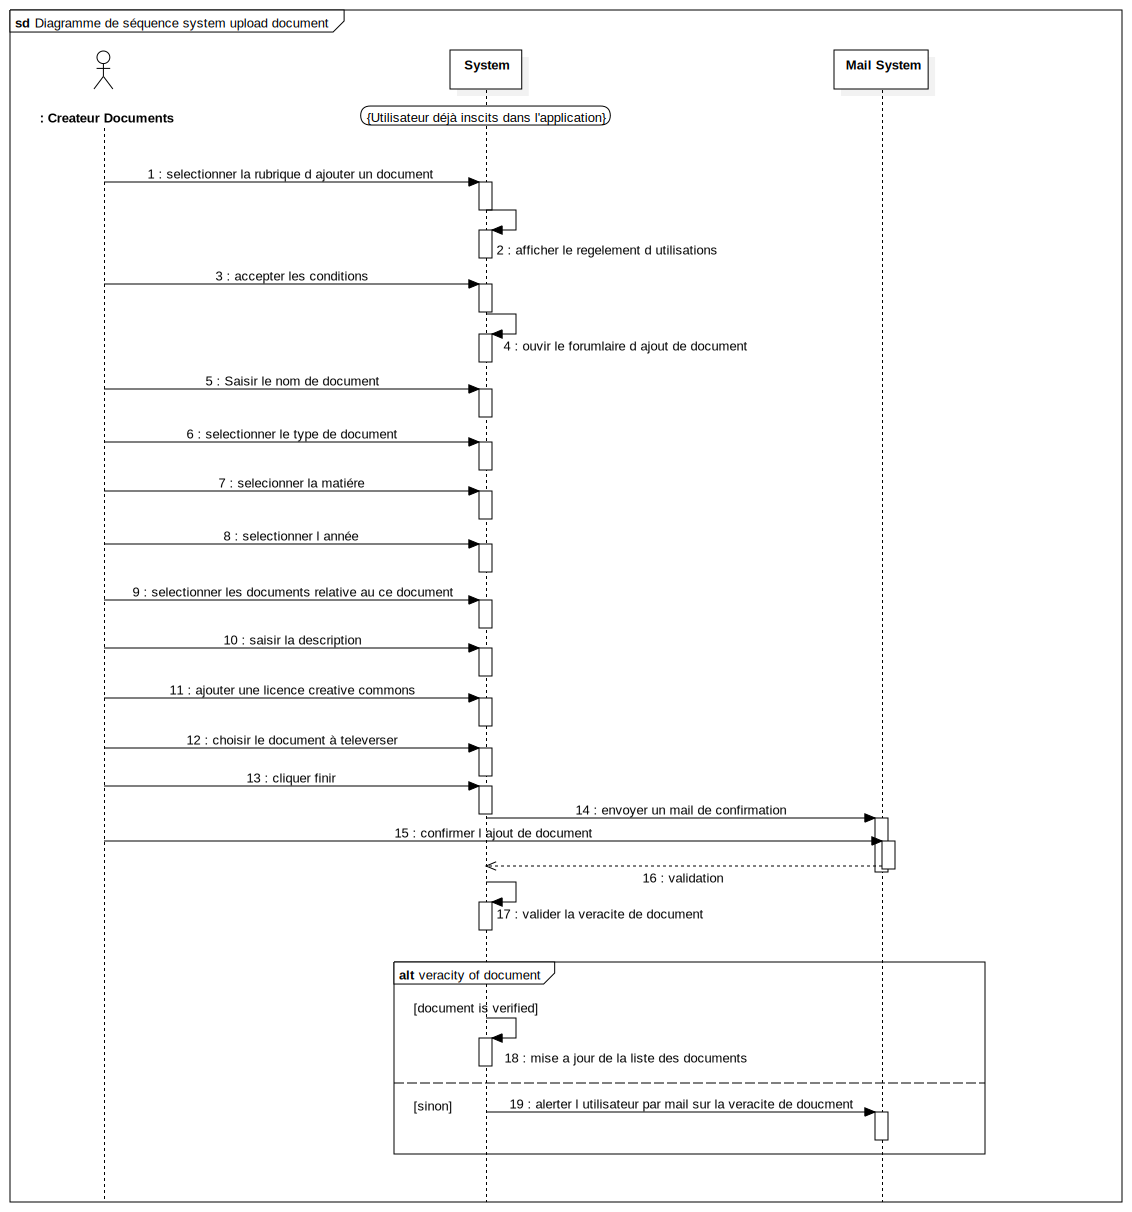
\includegraphics[width=1\textwidth]{Diagramme de séquence system upload document}
    \caption{Diagramme de séquence system upload document par UBooKer}
    \label{fig:diagrammedeséquencesystemuploaddocumentparubooker}
\end{figure}
\newpage
\subsection{Scénario Télécharger un documnet}
Nous avons représenter le scénario de téléchargement d'un document sur un maquéte pour faciliter l'intérprétation du comportement de systéme \ref{fig:diagrammedesséquencesystemdownloaddocumentparUbooker}

\begin{figure}[!hbtp]
    \centering
    \includegraphics[width=.88\textwidth]{Consulter un document}
    \caption{Maquéte download document par UBooKer}
    \label{fig:diagrammedesséquencesystemdownloaddocumentparUbooker}
\end{figure}
\newpage

\subsection{Scénario d'inscription dans un evenement}

Pour S'inscrire il est nécéssaire d'etre un UBooKer, et l'inscription réserve une place dans l'evenement.
Si l'event est payant, la page de payement s'ouvre pour payer l'inscription et automatiquement aprés une place sera reservé.
Le tableau qui représente les scénarios nominales, altérnatives de scénario d'inscription dans un evenemnt \ref{table:scénarios'inscrire dans un evenemnet par un ubooker} et le diagramme de séquence systeme est \ref{fig:diagramme de séquence inscription dans un evenet par ubooker}
\begin{table}[h!]
\begin{center}
\begin{tabular}{ |p{4cm}|p{11cm}|  }
 \hline
 \multicolumn{2}{|c|}{Scénario s'inscrire dans des events} \\
 \hline
 Titre & Inscrire dans des evenements\\
 \hline
 Acteur& UBooKer \\
 \hline
 Précondition   & \begin{itemize} 
 \item Le UBooKer n'est pas inscrit dans l'evenement
 \item L'evenement n'a pas atteint le nombre maximum d'inscription 
 \end{itemize}   \\
 \hline 
 Scénario nominale &   \begin{itemize}
 \item UBooKer clique sur s'inscrire
 \item UBooKer rempli les informations pour confirmer son identité
 \item UBooKer soumet le formulaire
 \item UBooKer recoit un alerte de reussite d'inscription
\end{itemize}   \\
 \hline
 Scénarios altérnatives & \begin{itemize}
 \item Si le lien vers l'inscription de l'evenement n'est pas dans UBooK: le UBooKer est redirigé vers ce lien,
 \item Si les informations soumet ne sont pas correcte, un message d'alerte indique il y'a un erreu dans l'entrée des coordonées
\end{itemize}   \\
 \hline
 Scénarios d'erreurs &  \begin{itemize}
 \item Si le UBooKer a quité la page d'inscription avant soumession : 
 aucune modification pour le utilisateur ni l'evenement
\end{itemize}   \\
 \hline
 Postconditions & Une place réservé dans l'evenement. \\
 \hline
\end{tabular}
\caption{Scénario S'inscrire dans un evenement par un UBooKer}
\label{table:scénarios'inscrire dans un evenemnet par un ubooker}
\end{center}
\end{table}

\begin{figure}[hbtp]
    \centering
    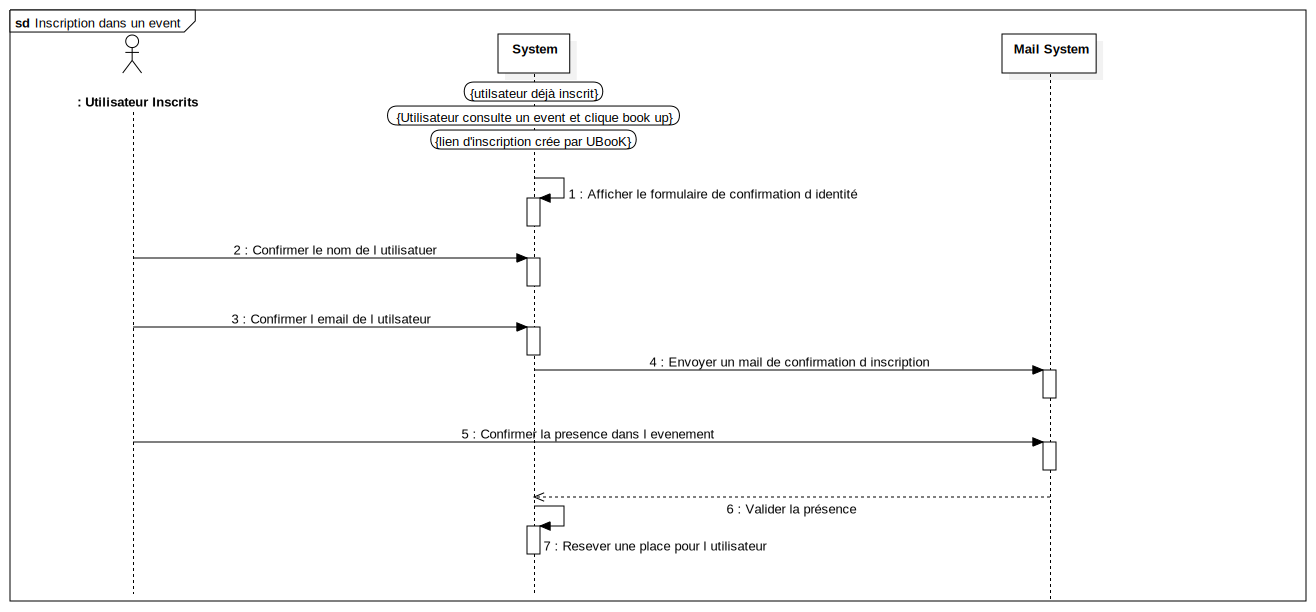
\includegraphics[width=1\textwidth]{Diagramme de séquence Inscription dans un event}
    \caption{Diagramme de séquence Inscription dans un event par UBooKer}
    \label{fig:diagramme de séquence inscription dans un evenet par ubooker}
\end{figure}
\newpage

\subsection{Scénario de gestion de ses evenements}

Pour ajouter un evenement, l'utilisateur doit etre un UBooKer, si l'utilisateur est indépendant de tous les organismes universitaires alors il doit payer pour afficher l'evenement, mais s'il est sous la supervision d'un organisme universitaires alors un mail de vérification sera envoyé vers ce derniér pour valider l'ajout gratuite.
Pour les autres gestion : la modification, la suppression et le suivie des inscriptions et limité sur le propriétaire de l'evenement.
Voir le tableau \ref{tableau:scénario ajouter un evenemnt par ubooker} pour les scénarios nominale ,altéranatives pour l'ajout d'un evenement, Pour le diagramme de séquence system voir \ref{fig:diagramme de séquence d'ajouter un event par ubooker}, et les maquétes pour l'ajout de l'evenement sont \ref{fig:maqutétes Ajout Evenement}

\begin{table}[h!]
\begin{center}
\begin{tabular}{ |p{4cm}|p{11cm}|  }
 \hline
 \multicolumn{2}{|c|}{Scénario Ajouter un evenement} \\
 \hline
 Titre & Ajouter un evenement\\
 \hline
 Acteur& UBooKer \\
 \hline
 Précondition   &  L'utilsateur est inscrit dans l'applicatoin UBooK   \\
 \hline 
 Scénario nominale &   \begin{itemize}
 \item UBooKer rempli les informations nécéssaire de l'evenement
 \item UBooKer soumet le formulaire
  \item L'evenement s'ajout mais privée pour le UBooKer
 \item L'organisme supérieur de UBooKer recoit un mail de vérification d'ajout d'evenement
 \item L'organisme supérieur de UBooKer confirme l'ajout d'evenement
 \item Un mail d'ajout avec succés envoyé vers le UBooKer
 \item l'evenement se mise à jour en publique
\end{itemize}   \\
 \hline
 Scénarios altérnatives & \begin{itemize}
 \item Si il y'a un champs nécéssaire n'est par rempli : le bouton de soumession est bloqué
 \item L'organisme supérieur de UBooKer n'a pas confirmé l'ajout : l'evenement reste privé avec possibilité de payement pour le rendre publique
  \item Le UBooKer est indépendants des organismes inscirts dans l'applicatoin : le UBooKer est redirigé vers la page de payement, pour finaliser l'ajout de l'evenement.
\end{itemize}   \\
 \hline
 Scénarios d'erreurs &  \begin{itemize}
 \item Si le UBooKer a quité la page d'ajout avant soumession : 
 aucune ajout s'effectue
\end{itemize}   \\
 \hline
 PostConditions & Le UBooKer est redirigé vers la page de consultation d'evenement. \\
 \hline
\end{tabular}
\caption{Scénario Ajouter un evenement par UBooKer}
\label{tableau:scénario ajouter un evenemnt par ubooker}
\end{center}
\end{table}

\begin{figure}[hbtp]
    \centering
    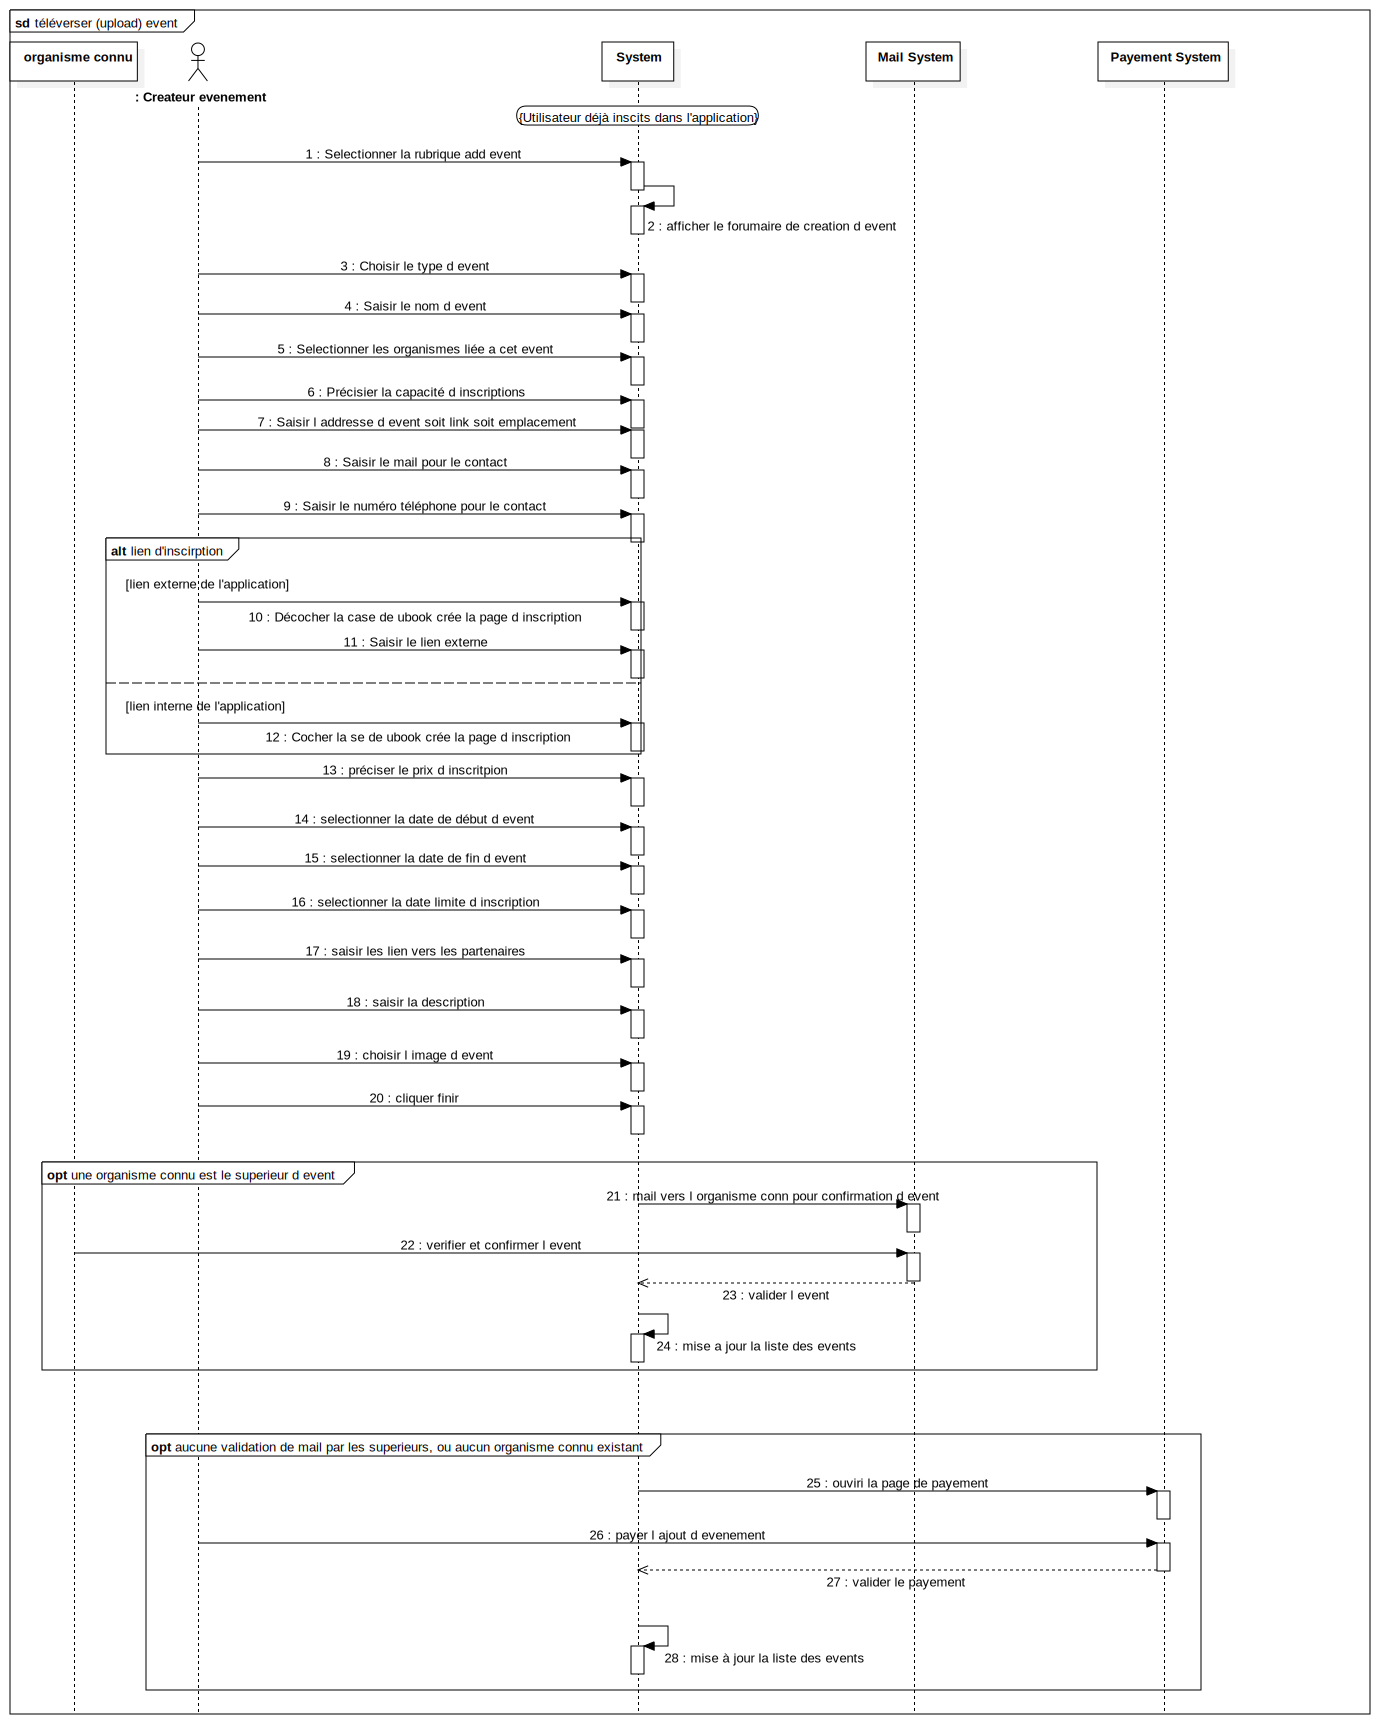
\includegraphics[width=1\textwidth]{téléverser (upload) event}
    \caption{Diagramme de séquence d'ajouter un event par UBooKer}
    \label{fig:diagramme de séquence d'ajouter un event par ubooker}
\end{figure}
\newpage

\begin{landscape}
\begin{figure}
     \centering
     \begin{subfigure}[b]{0.7\textwidth}
         \centering
         \includegraphics[width=\textwidth]{Add Event}
     \end{subfigure}
     \begin{subfigure}[b]{0.5\textwidth}
         \centering
         \includegraphics[width=\textwidth]{select university organisms}
     \end{subfigure}
     \caption{Maquétes Ajout Evenement Par UBooKer }
     \label{fig:maqutétes Ajout Evenement}
\end{figure}
\end{landscape}


\newpage
\subsection{Scénario Consulter un evenement}
Pour la consultation d'un evenement, l'internaute ouvre la rubrique event et choisi le type d'evenemnt qui'il en train de chercher, soit Jounrée soit certification soit compétition soit formation. Il trouve les récentes evenements affichés en grille. Il peut chercher dans la barre de recherche ou faire son filtrage, méme changer le type d'affichage en liste. Voir la maquéte \ref{fig: maqwakahow}
\begin{figure}[hbtp]
    \centering
    \includegraphics[width=.88\textwidth]{Consulter Event}
    \caption{Diagramme de séquence system consulter evenement par Internaute}
    \label{fig: maqwakahow}
\end{figure}
\newpage

\begin{landscape}
\newgeometry{left=1cm,right=0cm,bottom=0cm}
\section{Diagramme de classe analyse}
Dans ce diagramme on modélise les entités de l'application, et cette répresentation va étre le shéma dans la partie ingénieurie de base de donnée. Voir \ref{fig:diagrammedeclasseanalyse}	
\begin{figure}[hbtp]
    \centering
    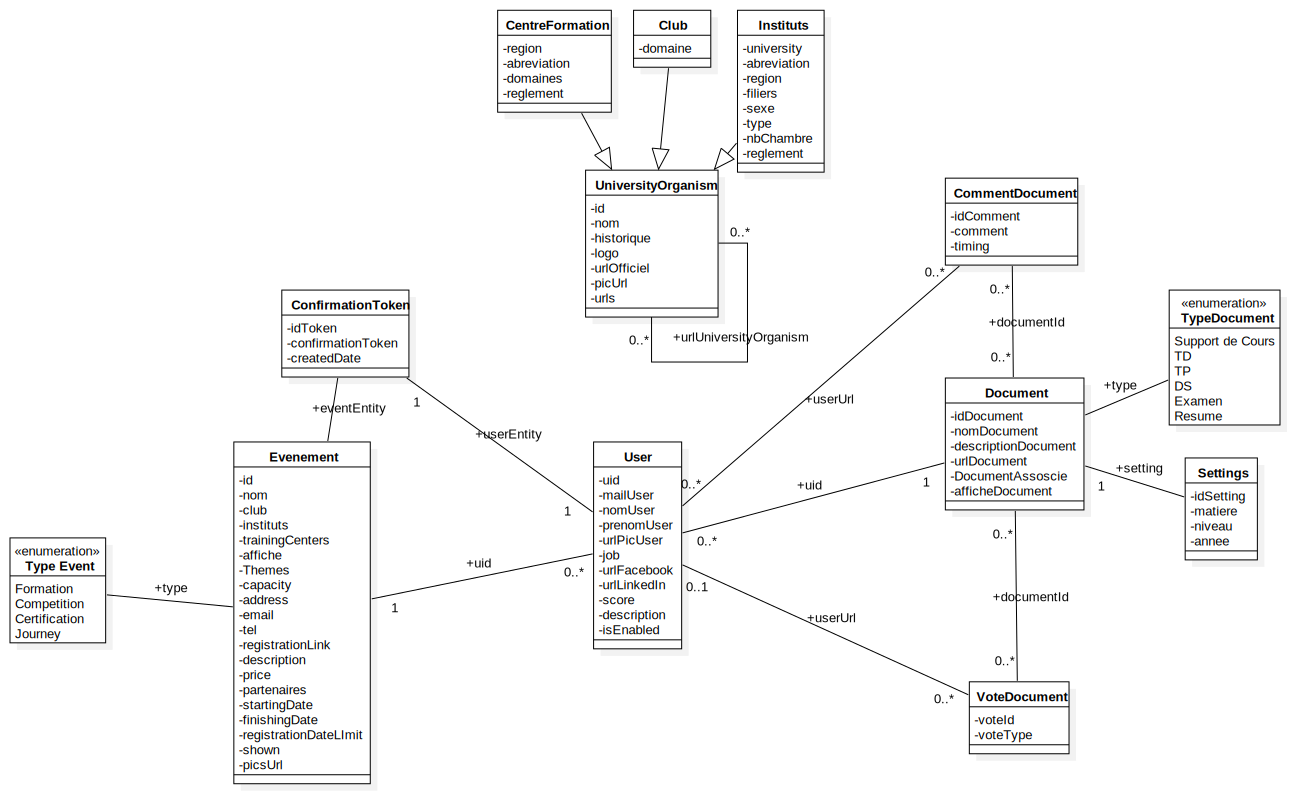
\includegraphics[width=1.1\textwidth]{AnalyseClassDiagram}
    \caption{Diagramme de classe d'Analyse}
    \label{fig:diagrammedeclasseanalyse}
\end{figure}
\end{landscape}
\restoregeometry
\newpage
\chapter{Conception}

Dans ce chapitre, nous présentons la partie ingénieurie de l'application.
\\

Dans ce projet, nous divisons l'application sur trois grandes parties: \\
- La partie Front End pour toutes les vues, nous choisissons le couleur rouge pour cette partie
- La partie Back End pour les controlleurs, nous choisissons le couleur bleu pour cette partie
- La partie Model qui répresente la couche Entity , nous choisisson le couleur vert pour cette partie.
\\

Commencons par le diagramme de Package \ref{fig:diag package} ou on modélise l'intéraction entre les diférentes parties, puis présentons le diagramme de classe conception sur deux figures la premiére représente la relation entre l'utilisateur et les documents \ref{fig:classe analyse 1}, la deuxiéme représente la relation entre l'utilisateur avec les evenements \ref{fig:classe analyse 2}, ensuite nous etudions quelques diagrammes de séquences objets qui sont :\\ \\
- Rechercher un document\ref{fig:diagramme de séquence liste documents}\\
- Téléverser un document\ref{fig:diagramme de séquence upload document}\\
- S'inscrire dans un evenement\ref{fig : diagramme de séquence inscription event}\\

\begin{landscape}
\newgeometry{left=1cm,right=0cm,bottom=0cm}
\section{Diagramme de Package}
\begin{figure}[hbtp]
    \centering
    \includegraphics[width=.8\textwidth]{Diagramme de Package}
    \caption{Diagramme de Package}
    \label{fig:diag package}
\end{figure}
\restoregeometry
\end{landscape}
\begin{landscape}
\newgeometry{left=1cm,right=0cm,bottom=0cm}
\section{Diagramme de classe conception}
\subsection{Relation UBooKer et Document}
\begin{figure}[hbtp]
    \centering
    \includegraphics[width=.9\textwidth]{Diagramme de Classe Conception pour les documents}
    \caption{Diagramme de classe d'Analyse}
    \label{fig:classe analyse 1}
\end{figure}
\end{landscape}
\restoregeometry
\begin{landscape}
\newgeometry{left=1cm,right=0cm,bottom=0cm}
\subsection{Relation UBooKer et Evenement}
\begin{figure}[hbtp]
    \centering
    \includegraphics[width=1\textwidth]{Diagramme de Classe Conception d'event}
    \caption{Diagramme de classe d'Analyse}
    \label{fig:classe analyse 2}
\end{figure}
\end{landscape}
\restoregeometry

\begin{landscape}
\newgeometry{left=1cm,right=0cm,bottom=-2cm}
\section{Diagrammes de séquences objets}
\subsection{Diagramme de séquence objet Rechercher un document}
\begin{figure}[hbtp]
    \centering
    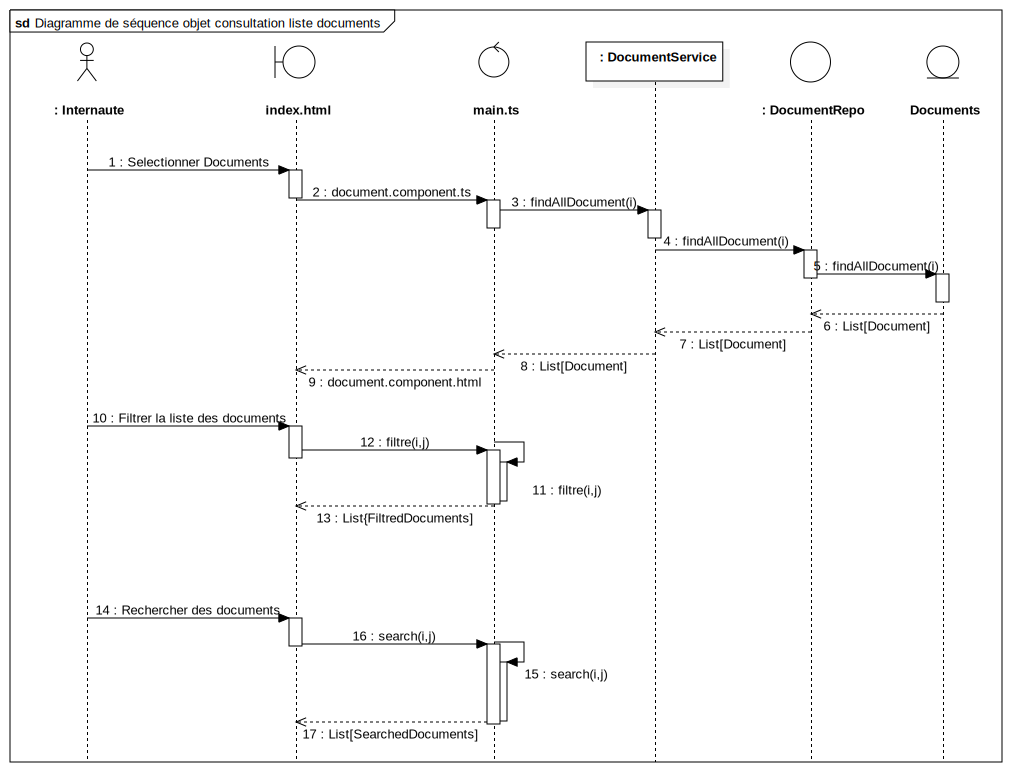
\includegraphics[width=1.1\textwidth]{Diagramme de séquence objet consultation liste documents}
    \caption{Diagramme de séquence objet consultation liste documents}
    \label{fig:diagramme de séquence liste documents}
\end{figure}
\end{landscape}
\restoregeometry
\begin{landscape}
\newgeometry{left=1cm,right=0cm,bottom=-2cm}
\subsection{Diagramme de séquence objet Téléverser un document}
\begin{figure}[hbtp]
    \centering
    \includegraphics[width=1.1\textwidth, height=.6\textwidth]{Diagramme de séquence objet upload document}
    \caption{Diagramme de séquence objet upload document}
    \label{fig:diagramme de séquence upload document}
\end{figure}
\end{landscape}
\restoregeometry
\begin{landscape}
\newgeometry{left=1cm,right=0cm,bottom=0cm}
\subsection{Diagramme de séquence objet S'inscrire dans un evenement}
\begin{figure}[hbtp]
    \centering
    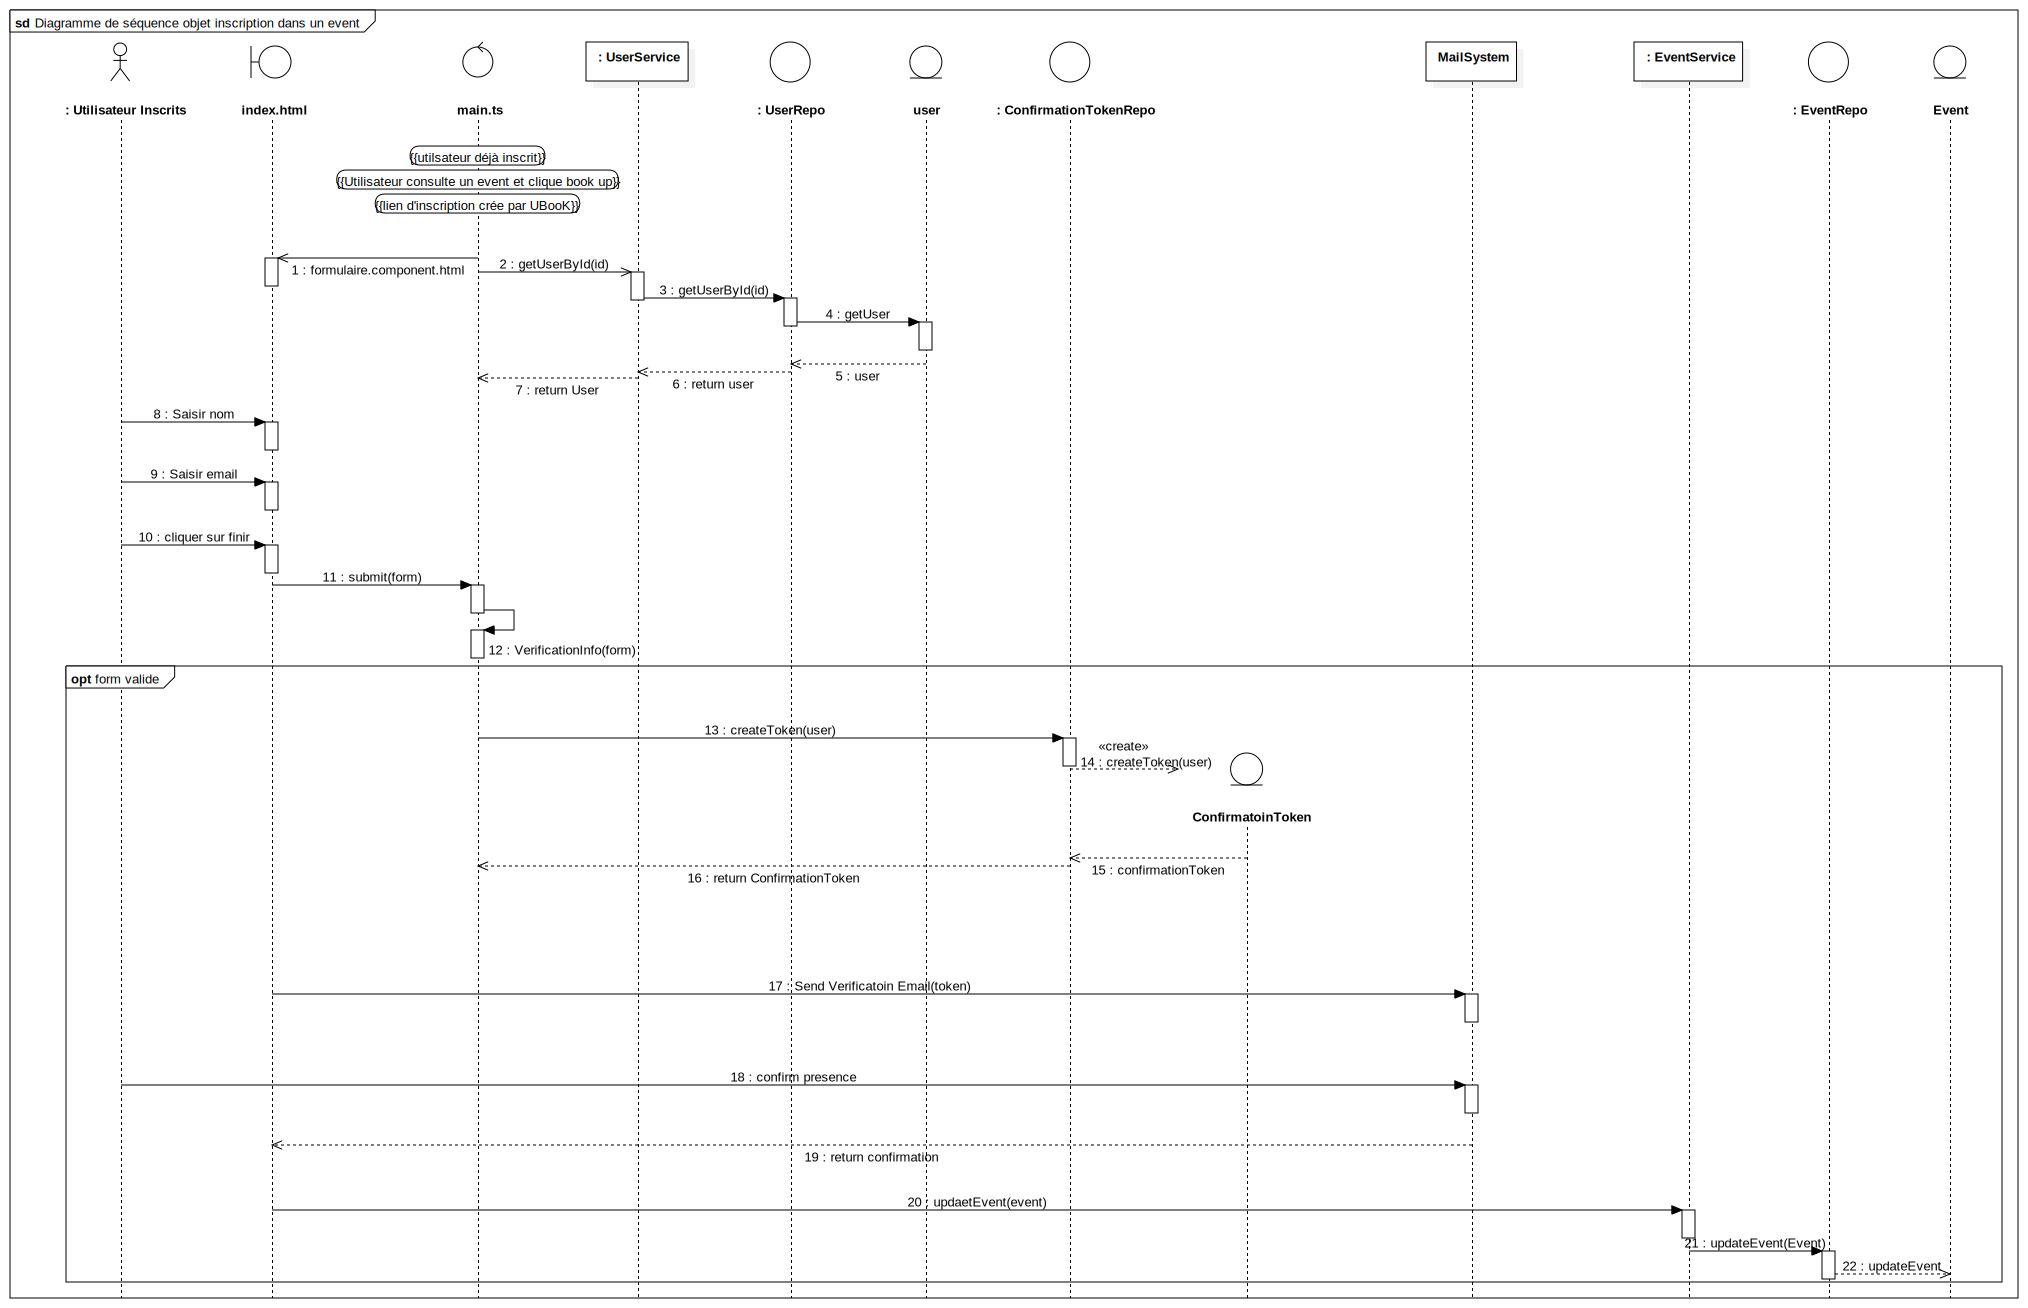
\includegraphics[width=1.1\textwidth]{Diagramme de séquence objet inscription dans un event}
    \caption{Diagramme de séquence objet inscription dans un event}
    \label{fig : diagramme de séquence inscription event}
\end{figure}
\end{landscape}
\restoregeometry


\newpage
\chapter{Realisation et déveleoppement}
\section{Environnement de travail}

Dans cette section, nous presentons les technologies utilisés pour la réalisation de projet UBooK.

\subsection{Les languages de programmations et les Framewroks}

\subsubsection{Framework Spring Boot}

Spring Boot est un framework de développement JAVA Entreprise Edition (JEE). C'est une déclinaison du framework classique de Spring qui permet essentiellement de réaliser des microservices (ce sont la majeure partie du temps des services web qui sont regroupés en API)\cite{24}.\\
Nous avons choisis Spring Boot(v 2.5.3) avec le jdk1.8 comme notre technologie Back End pour l'infrastructure logiciel associé aux dépendences :
\begin{itemize}
\item Spring Boot Starter Web : Un outil pour lancer le serveur web sur un port.
\item Lombok : Un outil pour génerer les Getters et les setters automatiquement
\item Spring Boot Starter Test : Un outil pour lancer tests sur le projet Spring.
\item Spring Boot Starter Data JPA : Un outil pour faciliter les requetes SQL 
\item Spring Boot Starter Mail : Un outil pour envoyer des emails à travers Spring Boot
\item FreeMarker : Un outil pour personalisé les emais avec le code html et css.
\end{itemize}

\subsubsection{Framework Angular}
Angular est un framework d'application Web gratuit et open source basé sur TypeScript, dirigé par l'équipe Angular de Google et par une communauté d'individus et d'entreprises. Angular est une réécriture complète de la même équipe qui a construit AngularJS.\cite{25}\\
Nous avons choisis Angular (v 12.2.6) de TypeScript (v 4.0.3) depuis le package manager npm (v 8.4.1) comme Front End pour l'infrastructure logiciel.

\subsubsection{Python}

le Python est un langage de programmation caractérisé par sa polyvalence : il est utilisé pour le développement web, l’IA, le machine learning, les systèmes d’exploitation, le développement d’applications mobiles, les jeux vidéo et bien d’autres.
Nous avons choisis Python comme un outil de vérification de véracité des documents comme indiqué dans la partie 2 (vers une modéle de véracité).

\subsection{Les systémes gestions base de données} 

\subsubsection{MySql}

MySQL est un système de gestion de base de données relationnelle open source. Nous avons utilisé MySql (version 8.0.28) comme notre systéme de gestion de base de données relationnelle.

\subsubsection{Framework Firebase}

Firebase est une plateforme développée par Google pour créer des applications mobiles et web. C'était à l'origine une société indépendante fondée en 2011. En 2014, Google a acquis la plate-forme et c'est maintenant leur offre phare pour le développement d'applications\cite{26}.\\
Nous avons utilisé Firebase comme un outil back end pour bénéficier de ces services d'authentification avec les application Google, Facebook, Twitter, LinkedIn.

\subsection{Outils Pour la modélisation, spécification et conception}

\subsubsection{StarUml}

StarUML est un logiciel de modélisation UML (Unified Modeling Language) open source. Étant simple d’utilisation, nécessitant peu de ressources système, supportant UML 2, ce logiciel constitue une excellente option pour une familiarisation à la modélisation\cite{27}.\\
Nous avons utilisé le logiciel StarUml pour modéliser les diagrammes UML de spécification et de conception.
\subsubsection{Blasamiq}

Balsamiq est un logiciel de conception de wireframes qui permet aux équipes de créer des maquettes et des prototypes interactifs, mais aussi de réaliser des tests utilisateurs. L’outil est destiné à tous ceux qui ont besoin de créer des wireframes, et son utilisation ne requiert pas d’expérience particulière dans le webdesign\cite{28}.\\
Nous avons Utilisé Balsamiq comme un outils pour faire la conception graphique, et modéliser les maquétes.

\subsection{Editeurs de textes}


\subsubsection{Framework JetBrains}

JetBrains est un éditeur de logiciels pour développeurs. Nous choisissons de travailler sur les editeurs de code de JetBrains qui sont : 
\begin{itemize}
\item Intellij (Editeur de texte pour Java)
\item WebStrom (Editeur de texte pour le Web (Angular, Html, Css, Javascript)
\item Pycharm (Editeur de texte pour Python
\end{itemize}


\subsubsection{Latex}

LaTeX (dont le logo est \LaTeX{}) est un langage et un système de composition de documents. Il s'agit d'une collection de macro-commandes destinées à faciliter l'utilisation du « processeur de texte » TeX de Donald Knuth\cite{29}.\\
Nous utilisons l'outil Latex pour ecrire les rapports.

\subsection{Sytéme de contrôle}

\subsubsection{Git et GitHub}

Git est de loin le système de contrôle de version le plus largement utilisé aujourd'hui. Git est un projet open source avancé, qui est activement maintenu\cite{30}.\\
GitHub is a for-profit company that offers a cloud-based Git repository hosting service. Essentially, it makes it a lot easier for individuals and teams to use Git for version control and collaboration\cite{31}.\\
Nous avons utilisé Git et Github comme un systéme de controle de version et de superviser l'avancement de projet.

\subsection{Systéme d'exploitation}

\subsubsection{Linux Ubuntu}

UBunut est un système d’exploitation GNU/Linux fondé sur Debian. Il est développé, commercialisé et maintenu pour les ordinateurs individuels (desktop), les serveurs (Server) et les objets connectés (Core) par la société Canonical\cite{32}.\\
Nous avons utilisé Ubunut version 20.04.4 LTS comme l'environnement de développement de l'application.
\newpage
\section{Résultat}

Dans cette section nous présetons quelques interfaces développés, ou nous presentons le design choisi, et nous montrons le bon suivi des maquétes.\\
Nous avons choisis les deux interfaces, Téléverser un document par UBooKer \ref{fig : televerser doc} et comme résultat de téléversement nous allons consulter ce document ajouté à traver l'interface de consultation de son documnet par UBooKer \ref{fig : consultatoin doc}

\begin{figure}[hbtp]
    \centering
    \includegraphics[width=1\textwidth]{101}
    \caption{Téléverser un document par UBooKer}
    \label{fig : televerser doc}
\end{figure}
\begin{figure}[hbtp]
    \centering
    \includegraphics[width=1\textwidth]{16}
    \caption{Consultation de son document par UBooKer}
    \label{fig : consultatoin doc}
\end{figure}

\newpage

\chapter*{Conclusion}
Dans cette partie nous avons bien exploré l'infrastructure de l'application UBooK qui traite l'aspect ethic la véracité d'information.\\
Dans la prochaine partie on étudie la partie recherche vers un modéle de véracité pour les document educatifs et pour les evenements universitaires qui s'execute sur l'infrastructure développé.

\part*{Vers un modéle de véracité}
\addcontentsline{toc}{part}{Vers un modéle de véracité}
\chapter*{Introduction}
UBooK est un réseau sociale qui offre des services 
de la vie estudiantine. Elle possède un espace de gestion 
d'événement et un espace de partage des documents éducatifs. 
\\Un des grands challenges c'est que le plateforme respecte 
les ethics et surtout la véracité d'information publié pour 
les documents éducatifs et les événements universitaires.
\\Alors dans ce chapitre on va Passer
 par les événements, on va les définir, 
enumérer les différent types et la politique 
fréquemment utilisé. 
\\Puis on s'intéresse sur les documents éducatives, on va différencier entre les types des documents éducatives et leurs métadonnées, Enfin citons une des politique pour les documents les licences Creative Commons 
\\Après on stop sur la véracité où on comprend mieux le
 concept et comment elle influence les documents et les 
événements et pour réaliser cet aspect on va raccourcir vers 
l'intelligence artificiel et elle même utilise l'indexation 
comme outil pour finir la tâche, ou on va se concentrer sur 
les deux derniers en les définir et mentionner les différentes
 types et modèles.

\newpage
\chapter{Etat de l'art}
\section*{Introduction}

La Data Science, ou science des données, est un mélange disciplinaire entre la data inférence, le développement d’algorithme et la technologie, dont l’objectif est la résolution de problèmes analytiques complexes. Au cœur de ce grand mélange, on retrouve les données, les quantités massives d’informations brutes stockées dans les data warehouses des entreprises. Concrètement, la science des données permet d’utiliser les données de façon créative pour générer une valeur pour les entreprises.

\begin{figure}[hbtp]
    \centering
    \includegraphics[width=.5\textwidth]{dcbdml}
    \caption{Data Science : Machine Learning + Big Data}
    \label{aaa : a1}
\end{figure}

Comme illustré dans la figure ci-dessus \ref{aaa : a1}, nous pouvons déviser les sciences des données en deux grandes branches : Big Data et L'intéligence artificel. \\
Dans ce chapitre nous présentons à la fois le Big Data et le l'artificial inteligence, et comment nous les exploitons pour réaliser la véracité pour les documents et les evenements, à travers les anciens travaux, et terminons vers notre modéle pour répondre à ce besoin.

\newpage
\section{Big Data}
L’explosion quantitative des données numériques a obligé les chercheurs à trouver de nouvelles manières de voir et d’analyser le monde. Il s’agit de découvrir de nouveaux ordres de grandeur concernant la capture, la recherche, le partage, le stockage, l’analyse et la présentation des données. Ainsi est né le « Big Data ». Il s’agit d’un concept permettant de stocker un nombre indicible d’informations sur une base numérique\cite{33}. \\
Les mégadonnées nous pouvons les présenter sur plusieur axes, critéres, qui sont appelés apres les Vs de Big Data. \\
Le Big data présente maintenant 42V  selon\cite{34} parmi eux nous trouvons le Volume, la Vitesse, la Variété, la Véracité, la Variabilité, la Validité, la Vulnérabilité, la Volatilité, la Visualisation et le Valeur.
\subsection{Véracité}
Dans ce projet, nous intéréssons sur le V Numéro 4 la Véracité, comme une qualité d'information que nous traitons, pour avoir une meilleur résultat.
\\
‘‘C'est l'un des enjeux majeurs de l'exploitation des Big Data. Faux profils
sur les réseaux sociaux, fautes d'orthographe, fraudes … Il est nécessaire
de multiplier les précautions (recoupement et enrichissement des données)
pour minimiser les biais liés au manque de fiabilité du Big Data\cite{35}.\\

La véracité est le quatrième V du Big Data. Il s’agit de la qualité et de l’exactitude des données. Les données collectées peuvent comporter des éléments manquants, être inexactes ou ne pas fournir d’informations réelles et utiles. La véracité fait globalement référence au niveau de confiance dans les données collectées.

Les données peuvent parfois être confuses et difficiles à utiliser. Si elles sont incomplètes, . Un exemple tiré du domaine médical : si les données sur les médicaments que prend un patient sont incomplètes, la vie du patient peut être en danger.

La valeur et la véracité contribuent toutes deux à définir la qualité et les informations tirées des données. Dans un sens, c’est un facteur d’hygiène. En démontrant la véracité de vos données, vous montrez que vous avez porté un regard critique sur elles.

\subsubsection{Notion de véracité}
Qualité morale de celui/celle qui ne trompe pas ou qui n'en a pas l'intention; en partic., qualité de celui/celle qui se garde de l'erreur et s'emploie à l'éviter dans ses paroles ou dans ses écrits. Synon. bonne foi*, exactitude, franchise, sincérité, véridicité.\\
Caractère de ce qui est conforme à la vérité, à la réalité. Synon. authenticité, exactitude.\\
Souci, recherche de l'exactitude, de la fidélité au réel, notamment dans la création artistique et littéraire.\\
VÉRACITÉ, (Morale.) la véracité ou vérité morale dont les honnêtes gens se piquent, est la conformité de nos discours avec nos pensées ; c’est une vertu opposée au mensonge\cite{36}.\\

La véracité fait référence à la provenance ou à la fiabilité de la source de données, à son contexte et à son importance pour l'analyse qui en découle. Des réponses à ces questions sont nécessaires pour déterminer la véracité de ces informations. La connaissance de la véracité des données nous aide à mieux comprendre les risques associés aux analyses et aux décisions commerciales basées sur cet ensemble de données particulier.
\subsubsection{Véracité Pour les Documents}
La véracité dans les documents se fait à travers la 
conformité des métadonnées avec le contenu du document, 
en plus un document vide ou bien qui mentionne une information 
fausse alors il n'est plus vrai.
Par exemple un document de grammaire 
française, ne doit pas être vide ou son contenu est 
autour de la musique. Si ces conditions sont validés alors ce 
document est vrai. 
Aussi que la véracité est lié d'authenticité si l'auteur 
n'est pas celui le propriétaire de document alors aucune 
véracité existante.
\subsubsection{Véracité Pour les evenements}

La véracité pour les événements signifie que la certitude de 
déroulement de cet événement, en plus qu'il est bien conforme 
aux thématiques mentionnées. \\Mais la véracité ne se limite pas au
 événement lui même mais aussi les inscription aux evénement 
doit être vrai car on peut y avoir des faux inscritption pour 
les participants.
\section{Intéligence Artificiel}
\subsubsection{Notion d'IA}

L'intelligence artificielle (IA, ou AI en anglais pour Artificial Intelligence) consiste à mettre en œuvre un certain nombre de techniques visant à permettre aux machines d'imiter une forme d'intelligence réelle. L'IA se retrouve implémentée dans un nombre grandissant de domaines d'application.\\
Les domaines d'application de l'intelligence artificielle sont nombreux. Elle est présente dans les appareils photo des smartphones. En mode nocturne, elle permet d'adapter la colorimétrie à l'environnement, et de redonner à une façade éclairée son éclat originel pour le reproduire fidèlement sur votre cliché\cite{37}.\\

En termes simples, l'intelligence artificielle (IA) fait référence à des systèmes ou des machines qui imitent l'intelligence humaine pour effectuer des tâches et qui peuvent s'améliorer en fonction des informations collectées grâce à l'itération\cite{38}.\\

Il y'a qutare écoles en IA : 
\begin{itemize}
\item Penser comme des humains : Les efforts passionnats pour pousser les ordinateurs à penser d'en fabriquer des machines avec cerveaux au sens le plus latéral.(Haugeland, 1985)
\item Penser Rationnellement : L'etude des facultés mentales par l'élaboration des modéles mathématiques.(Charniak et McDermott, 1987)
\item Agir comme des humains : L'etude des moyens qui permettent aux ordinateurs de faire des choses qui pour le moment sont mieux faites par des hommes.(Rich et Knight, 1991)
\item Agir rationnellement : L'etude et la conception d'agents intelligents.(Poole, 1998)
\end{itemize}

\subsubsection{Notion de ML}

L'apprentissage automatique est une branche de l'intelligence artificielle
(IA) et de l'informatique qui utilise principalement des données et des
algorithmes pour imiter la manière dont les être humains apprennent, en
améliorant progressivement sa précision.
L'apprentissage automatique est une composante importante du domaine
en pleine expansion qu'est la science des données. Grâce à l'utilisation de
méthodes statistiques, des algorithmes sont entraînés à effectuer des
classifications ou des prévisions, ce qui permet de découvrir des
informations essentielles dans le cadre de projets d'exploration des
données. Ces informations permettent ensuite de prendre des décisions
dans les applications et les entreprises, et ont idéalement un impact sur les
principales métriques de croissance. Au fur et à mesure que le big data
poursuit son développement et sa croissance, les besoins en spécialistes
des données va augmenter, ce qui les obligera à contribuer à l'identification
des questions commerciales les plus pertinentes et, par conséquent, des
données permettant d'y répondre\cite{39}.\\


En machine learning il y’en a deux branches, l’apprentissage supervisé et non supervisé.
Ce dernier consiste à prédire par oui ou non (Vrai ou Faux) à une proposition ‘statement’ après un entraînement sur deux clusters. Son rôle est la plupart de différencier entre deux groupes. Les fameux modèles sont K-Means, CAH...
Et l’apprentissage supervisé lui même a deux sous branches le classification et la régression.
Pour le classification son but est de classifier et donner une famille ou un valeur brute pour une donnée, la plupart d’utilisation de classification et de prédire un type de donnée. Les fameux modèles sont : KNN, CNN,Arbre de décision…
Mais pour la régression et de donner un intervalle de valeur pour une donnée, la plupart d’utilisation de régression est dans la prédiction des valeur numérique, ou prédiction des pourcentages. Les fameux modèles sont : Linear Régression, Polynomial Regression...
\subsection{Scrapping}
\subsubsection{Notion de Scrapping}
La capture de données d’écran (screen scraping en anglais) est une technique par laquelle un programme récupère des données normalement destinées à être affichées par un dispositif de sortie vidéo (généralement un moniteur) afin d’en extraire des informations.\\

Il s’agit souvent de pages web dans lesquelles on souhaite récupérer des informations, mais il peut également s’agir de toute autre forme d’informations qui est formatée avant tout en vue d’être affichée sur un écran. Il peut également s’agir d’informations destinées à un terminal texte, ou encore d’un écran de téléphone cellulaire sur lequel les informations peuvent être analysées après y avoir été affichées par une autre application\cite{40}.\\

Recueillir des données sur le web est parfois compliqué et quand cela est possible, il est difficile de pouvoir les télécharger ou d’effectuer un copier-coller. Le web scraping est une technique permettant l’extraction des données d’un site via un programme, un logiciel automatique ou un autre site. L’objectif est donc d’extraire le contenu d’une page d’un site de façon structurée. Le scraping permet ainsi de pouvoir réutiliser ces données\cite{41}.\\

Le web scrapping est un outil d'extraction des données depuis autres WebSites, à travers un script, et une connaissance sur le structuration de web que nous voulons extraire des informations, nous pouvons réutiliser les données, et les exploiter pour satisfaire notre besoins.
\subsubsection{Modéles de scrapping}

Selons le site \cite{42} nous présentons quelques outils de web scrappig: 
\begin{itemize}
\item Beautiful Soup : c'est vraiment un bel outil pour les scrappers Web en raison de ses fonctionnalités de base. Cela peut aider le programmeur à extraire rapidement les données d'une certaine page Web. Cette bibliothèque nous aidera à extraire les données des fichiers HTML et XML. Mais le problème avec Beautiful Soup est qu'il ne peut pas faire tout le travail tout seul. cette bibliothèque nécessite des modules spécifiques pour fonctionner.
\item Selenium: Selenium est conçu pour automatiser les tests des applications Web. Il permet au développeur d'écrire des tests dans un certain nombre de langages de programmation populaires tels que C\#, Java, Python, Ruby, etc. Ce framework est développé pour effectuer l'automatisation du navigateur. Jetons un coup d'œil à l'exemple de code qui automatise le navigateur.
\item Scrapy: est un framework open source collaboratif qui permet d’extraire les données d’un site web de manière simple et rapide. Développé sous Python, Scrapy dispose d’une grande communauté qui n’hésite pas à créer des modules supplémentaires pour améliorer l’outil.
\item Webscraper: est une extension disponible sous Google Chrome qui permet d’extraire les données d’un site internet très rapidement. Web Scraper naviguera sur les sites choisis afin d’en extraire toutes les données. Les données collectées peuvent être exportées sous forme de CSV. L’extension vous permet également de scrapper plusieurs sites à la fois ou même les programmer.
\item PhantomBuster: Zéro code et des résultats. Voilà la promesse tenue de PhantomBuster. L’outil offre la possibilité d’extraire les données que vous souhaitez, mais aussi de créer des chaînes d’actions pour générer des pistes d’affaires, des audiences de marketing et une croissance globale. Phantombuster vous donne les outils et le savoir-faire nécessaires pour faire croître votre entreprise plus rapidement. Un outil que nous utilisons chez Wydden et que nous vous présentons dans notre formation Growth Marketing.
\item Octoparse :Un des pionniers du scraping web. L’outil Octoparse offre un interface « pointer-cliquer » qui signifie que toute personne qui sait naviguer peut scraper. Aucun code n’est nécessaire. Vous pouvez extraire de données de n’importe quel site web dynamique et récupérer des pages illimitées gratuitement.
\item ...
\end{itemize}

\subsection{Indexation}
\subsubsection{Notion D'indexation}
L'indexation automatique de documents est un domaine de l'informatique et des sciences de l'information et des bibliothèques qui utilise des méthodes logicielles pour organiser un ensemble de documents et faciliter ultérieurement la recherche de contenu dans cette collection.La multiplicité des types de documents (textuels, audiovisuels, Web) donne lieu à des approches très différentes, notamment en termes de représentation des données. Elles reposent néanmoins sur un socle de théories communes, telles que l'extraction de caractéristiques, le partionnement de données (ou clustering), la quantification, et plus généralement la recherche d'information\cite{43}.\\
En général, l'indexation fait référence à l'organisation des données selon un schéma ou un plan spécifique. En informatique, le terme a diverses utilisations similaires, notamment pour rendre les informations plus présentables et accessibles\cite{44}.\\

L'indexation des documents consiste à associer des mots clés et informations à chaque documents en fonction du plan de classement, afin de faciliter, ensuite, la recherche, l’accès et le traitement par les utilisateurs.

Alors l’indexation est un ensemble des méthodes et techniques pour l’acquisition, l’organisation, le stockage, la recherche et la sélection d’information pertinente pour un utilisateur

\subsubsection{Modéles D'indexation}
Le modéle de recherche d'information RI comprend la fonction de décision fondamentale qui permet
d’associer à une requête, l’ensemble des documents pertinents
à restituer.Il est étroitement lié au modèle de représentation des
documents et requêtes.\\
L’appariement requête-documents consiste à calculer un score,
supposé représenter la pertinence du document vis-à-vis de la
requête.\\
Ce score est souvent calculé à partir d’une fonction ou une
probabilité de similarité, en fonction du modèle utilisé, qui tient
compte du poids des termes dans les documents.
L’assignation d’un score de pertinence à un document permet
d’ordonner les documents renvoyés à l’utilisateur
Comme illustré dans \ref{aaa:a2} Nous allons presenter quelques modéles, que nous avons besoin aprés dans l'etude d'ature solutions existants. 
\begin{figure}[h]
    \centering
    \includegraphics[width=1\textwidth]{indexation}
    \caption{Classification des modèles selon la théorie}
    \label{aaa:a2}
\end{figure}

\begin{itemize}
\item Modéle Booléen : C’est le premier modèle de RI,
Introduit en 1983 par Salton et McGill, 1 er SRI commercial pour 3 décennies (60-90), Basé sur la théorie des ensembles et l’algèbre de Boole, L’interface d’interrogation de la plupart des moteurs de
recherche est basée sur les principes de ce modèle.\\
Il considère que les termes de l’index sont présents ou
absents d’un document\\
Les poids des termes dans l’index sont binaires : w i,j = \{0, 1\}\\
Un document est soit pertinent soit non pertinent pour une
requête donnée : Pertinence binaire, et jamais partielle.

\item Modéle Booléen Pondéré : Extension du modèle booléen en intégrant des
pondérations (dénotant la représentativité d’un terme
pour un document) \\
Fonction de correspondance non binaire (on se passe des
implications logiques) basée sur une similarité notée Sim

\item Modéle vectoriel : Dans des très grandes collections de documents, le
résultat de recherche pour une requête donnée dépasse
généralement la capacité des utilisateurs à examiner tous
les documents de l’ensemble retourné\\ Affecter un score (degré de similarité), à chaque document
relativement à une requête donnée : le document le plus
pertinent devrait avoir le score le plus élevé.
\item ...
\end{itemize}
\subsection{ML \& Documents}
Les fameux modèles qui traitent la véracité des document utilisent le traitement automatique de langage naturel TAN :\\ Le traitement automatique du langage naturel imite la compréhension
humaine des mots et des phrases et permet maintenant aux modèles
d'apprentissage automatique de traiter de grandes quantités d'informations
avant de fournir des réponses précises aux questions qui leur sont posées.
L'utilisation du TAN permet de comprendre le contenu du document et vérifier sa véracité.
\\Autre modèles qui traitent la véracité sont la classification des documents par l'apprentissage automatique, on mentionne en titre d'exemple KNN, Arbre de décision, Naive Bayes
Dans la section suivante on suit les travaux anciens et leurs modèles qui traitent la véracité des documents.
\subsection{Scrapping \& Evenement}
Le web scraping (parfois appelé harvesting) est une technique
d'extraction du contenu de sites Web, via un script ou un programme, dans
le but de le transformer pour permettre son utilisation dans un autre
contexte, par exemple le référencement \cite{45}\\
le grattage du web permet de chercher un ensemble 
d’information sur des
sites bien spécifiques, c’est modèle d’IA qui parcours 
le web sémantique et
vérifie les balises HTML.
Les meilleurs bibliothèques dans le web scraping sont :
Scrapy (Python), BeautifulSoup (Python), Requests (Python), LXML
(Python), Selenium (Python), Jsoup (JAVA) ...

Le grattage du web permet de récupérer les vraies événements 
en cherchant dans les sites et les pages d'événement 
confiants

\section{Travaux anicennes}

\subsubsection{Feuille de route}

Dans cette partie on va s’intéréssé sur les travaux anciens qui est autours la véracité. 
En premier lieu on étudie les modéles sur la véracité d’information de facon générale
En second lieu on étudie les modéles sur la véracité principalement des documents

\subsection{Modéles de Recherche sur la véracité}

\subsubsection{Système d’aide à la décision pour la véracité des données dans le contexte de Big Data}

Comme la fiabilité des données est un challenge concrétisé par la
dimension de véracité dans le contexte de Big Data, et afin d’extraire des
données fiables à partir des systèmes d’information ou les données peuvent
incomplète, imprécisé, vague,…etc. Ce travail répond à l’objectif de la
création d’un système basé sur la théorie de Rough sets* de véracité de
données dans un contexte de Big data.
\\
*La théorie des ensembles approximatifs (RST) est une approximation
formelle de la théorie des ensembles conventionnelle qui prend en charge
les approximations dans la prise de décision. Cette approche peut extraire
des connaissances d'un domaine problématique de manière concise et
conserver le contenu de l'information tout en réduisant la quantité de
données impliquée\cite{46}.\\ \\



\subsubsection{Modèle probabiliste avec support mutuel des valeurs similaires}

Basé sur l’analyse bayésienne, TruthFinder (Yin et al., 2008) calcule la
fiabilité de l’information donnée par une source. Il s’appuie sur l’honnêteté
de la source d’information et suit l’heuristique selon laquelle si les valeurs
fournies sont essentiellement vraies pour de nombreux cas, alors elles
seront aussi probablement vraies pour d’autres cas. Mais dans notre cas ce n’est plus fonctionnel car on cherche à un modèle ou le source est unique.
Et l’information vient d’un seul source, ne peut par étre des sources
différents, en respectant la non redondance\cite{47}.


\subsubsection{Découverte de la vérité par corroboration d’informations}

C’est un ensemble de trois algorithmes proposés dans (Galland et al.,
2010) : COSINE, 2 ESTIMATES et 3-ESTIMATES. COSINE initialise la
fiabilité de chaque valeur et de chaque source. Il calcule de façon itérative
la fiabilité d’une source comme une fonction linéaire de sa fiabilité
précédenteMais dans notre cas ce n’est plus fonctionnel car on cherche à
un modèle ou le source est unique. Et l’information vient d’un seul source,
ne peut par étre des sources différents, en respectant la non redondance\cite{48}.

\subsubsection{Modèle de vérité latente}

Ce modèle utilise les réseaux bayésiens pour estimer la fiabilité de
l’information. " Latent Truth Model " (LTM) est proposé dans (Zhao et al.,
2012). Il se base sur deux hypothèses :
\\— les données doivent contenir un seul attribut avec une valeur atomique ;
\\— la gestion de plusieurs valeurs vraies pour le même attribut.
Pour chaque source, LTM considère les probabilités à priori pour qu’elle
soit un vrai positif ou un faux positif avec des erreurs négatives. Enfin, les
valeurs dont le degré de fiabilité est supérieur à 0.5 sont considérées
comme vraies. Il faut noter que le LTM peut ne pas détecter des valeurs
vraies pour certains attributs\cite{49}.
\subsubsection{Découverte de la vérité par estimation de la vraisemblancemaximale}

Basée sur la maximisation de la vraisemblance pour quantifier la fiabilité
des sources et la justesse des valeurs, " Maximum Likelihood Estimation "
(MLE) est proposé dans (Wang et al., 2012). MLE traite seulement les
observations booléennes positives et ignorent celles négatives. Dans son
algorithme, MLE initialise les paramètres des sources :
\\— a(s) probabilité pour que la source s signale une valeur vraie et elle est
effectivement vraie
\\— b(s) probabilité pour que la source s signale une valeur vraie alors
qu’elle est en réalité fausse.
De façon itérative, MLE calcule la probabilité conditionnelle d’une valeur
v d’être vraie sur la base des probabilités (a(s), b(s)) de sa source et celle
des sources ne fournissant pas la valeur v. Ensuite la confidence de chaque
valeur est calculée itérativement. Après cela, MLE procède à la mise à jour
des probabilités (a(s), b(s)) de chaque source. Les itérations s’arrêtent à la
convergence de a(s) et b(s). Une importante observation faite dans les
expériences de l’article (Waguih and Berti-Equille, 2014) permet de dire
que MLE ne peut pas être utilisé avec de grands nombre de sources
(>5000).
Mais dans notre cas ce n’est plus fonctionnel car on cherche à un modèle
ou le source est unique. Et l’information vient d’un seul source, ne peut
par étre des sources différents, en respectant la non redondance\cite{50}.

\subsubsection{Découverte de la vérité avec dépendance de sources par copie}

Ici, nous parlerons des algorithmes de recherche de vérité qui tiennent
compte de la relation qui existe entre sources. DEPEN est le premier
proposé dans (Dong et al., 2009). C’est un modèle bayésien de recherchede vérité qui prend en considération les relations de copie qui peuvent
exister entre les sources en pénalisant le vote d’une source si elle est
détectée comme étant la copie d’une autre source. Le calcul de la matrice
de dépendance entre les sources est très coûteux surtout lorsque les
données en entrée sont volumineuses ; c’est un des goulots d’étranglement
majeurs de DEPEN et ses extensions\cite{51}.

\subsubsection{Analyse de crédibilité latente}

LCA (" Latent Credibility Analysis ") est un modèle probabiliste proposé
dans (Pasternack and Roth, 2013). Il utilise aussi l’algorithme de
maximisation de la vraisemblance pour calculer la probabilité des valeurs
en regroupant les mêmes attributs d’un même objet en une même donnée
dans un ensemble d’exclusion mutuelle où il n’existe qu’un seul élément
vrai. LCA est une approche flexible et puissante pour modéliser le
problème de la crédibilité de l’information\cite{52}.
\subsubsection{Découverte de la vérité dans plusieurs domaines de sources contradictoires ayant des vérités multiples}

Ce modèle est un modèle probabiliste et bayésien à la fois, qui intègre le
score d’expertise de domaine et le score de confiance pour la
détermination de la vérité. DART (Domain AwaRe Truth Discovery) est un
modèle proposé dans (Lin and Chen, 2018). L’idée de base est la
construction d’un modèle, qui contient deux composantes intégrales : la
modélisation de l’expertise du domaine concernant la richesse des
données, et la modélisation de l’agrégation de la vérité à partir des
réponses de chaque source\cite{53}.
\subsubsection{Découverte de la vérité avec partitionnement des attributs}

Proposée dans (Lamine Ba et al., 2015), c’est une méthode de recherche de
vérité qui se base sur le partitionnement des attributs des objets. Son
objectif est donc d’estimer une partition optimale de l’ensemble des
attributs de telle sorte qu’en appliquant indépendamment n’importe quel
algorithme de recherche de vérité de référence sur chaque sous ensemble
de la partition, on maximisera la précision de cet algorithme. L’estimation
de la partition optimale dans ce cas se base seulement sur la qualité de
l’algorithme de recherche\cite{54}.


\subsubsection{Modèle probabiliste pour la découverte de la vérité avec des corrélations d’objets avec des contraintes}

Ce modèle probabiliste se base sur la corrélation entre les objets en tenant
compte de certaines contraintes qui lui sont fournies en entrée. "
Constrained Truth Discovery " (CTD) est proposé dans (Yang et al., 2019)
et formulé comme un problème d’optimisation sous contraintes. Le
processus de découverte de la vérité intègre les contraintes de type "
Denial Constraints (DCs) " (Chomicki and Marcinkowski, 2005) à l’aide
d’un formalisme basé sur la logique du premier ordre universellement
quantifié qui peut exprimer un grand nombre de relations effectives et
largement existantes entre les objets. Sur cette base les auteurs proposent
des algorithmes pour partitionner les objets en groupes disjoints en
générant des contraintes arithmétiques pour chaque groupe disjoint
séparément. Ensuite, les vraies valeurs des attributs des objets dans chaque
groupe disjoint sont dérivées en minimisant une fonction objective sous les
contraintes arithmétiques correspondantes\cite{55}.
\subsubsection{Vérification de faits par partitionnement de données}

Dans ce travail, nous intéresse la vérification de faits dans un domaine où
les données ont une structure inhérente qui n’est pas connue à l’avance.
Pour résoudre ce problème il a été conçu et proposé un algorithme, appelé
TD-AC, de partitionnement de données intelligent basé sur la méthode de
clustering des données des k-moyennes du domaine de l’apprentissage
automatique. Pour choisir la partition optimale, l’indice de silhouette a été
choisis. Ensuite, (OSIAS NOËL) a proposé une validation des
performances de l’algorithme. Pour ce faire, il l’a comparé à l’approche
proposée dans (Lamine Ba et al., 2015) et aux algorithmes de découverte
de la vérité standards sur des jeux de données synthétiques, semi
synthétiques et réelles. Enfin, (OSIAS NOËL) a montré que TD-AC a une
complexité en temps comparable à celle des algorithmes standards
contrairement à l’algorithme brute force dans (Lamine Ba et al., 2015).
Cependant, nous avons observé que lorsque le jeu de données est
caractérisé par beaucoup de valeurs, cet approche est moins
performante : ceci à cause de l’utilisation d’une matrice creuse comme
entrée de l’algorithme de clustering entraînant une difficulté à trouver la
partition optimale\cite{56}.
\subsection{Modéles de Recherche sur la véracité pour les documents educatifs}

\subsubsection{Incorporation de phrases (SIF)}

Les travaux qui ont combinaient l'incorporation de mots en utilisant des
opérations sur des vecteurs et des matrices pour dériver l'incorporation de
phrases ou de phrases. Les résultats ont montré que l'exploitation des
vecteurs par multiplication par coordonnées permet d'obtenir de très
bonnes performances dans les opérations binaires étudiées. Et concentré
sur les représentations distribuées des phrases. Ils nécessitaientgénéralement une analyse syntaxique et il a été démontré que le résultat
fonctionnait pour les représentations au niveau de la phrase. Une autre
approche a mis en place un algorithme non supervisé pour apprendre les
représentations distribuées de phrases ou de documents. Leurs expériences
ont indiqué que leur méthode était compétitive avec les méthodes de
pointe\cite{57}.

\subsubsection{Analyse syntaxique}

L'analyse syntaxique est l'une des technologies de base du traitement du
langage naturel et la pierre angulaire d'une compréhension approfondie du
langage. La tâche de l'analyse syntaxique est d'identifier les composants
syntaxiques contenus dans la phrase et la relation entre ces composants, en
utilisant généralement des arbres d'analyse pour représenter les résultats de
l'analyse syntaxique\cite{58}.
\subsubsection{Calcul de l'incorporation de phrases en fusionnant l'arbre d'analyse syntaxique et l'incorporation de mots}

L'article propose une méthode d'incorporation de phrases basée sur les
résultats de l'arbre d'analyse syntaxique et des vecteurs de mots. L'ordre de
fusion des nœuds dans l'arbre d'analyse garantit que la méthode est capable
de conserver l'ordre des mots dans les phrases. Et (Yong Wang, Shuixiu
Wu) considérent les balises de l'arbre d'analyse comme des paramètres de
poids, qui capturent les informations syntaxiques dans l'incorporation de
phrases. Ainsi, la méthode proposée a le potentiel de surmonter la faiblesse
des méthodes existantes. De plus, il est rapide à calculer et à apprendre les
paramètres, en plus d'obtenir des performances meilleures ou comparables
que SIF traditionnel sur diverses tâches de similarité textuelle. De plus, il ya aussi quelques problèmes dans la méthode qui devraient être améliorées.
Par exemple, l'apprentissage des paramètres doit être optimisé, comme la
conception d'une fonction cible d'apprentissage non supervisée pour
obtenir de meilleures performances\cite{59}.
\subsubsection{Conclusion vers notre modéle}
Nous avons présenté ci-dessus quelques récents travaux sur les méthodes de recherche de vérité.
Ces méthodes se basent dans la majeure partie des cas sur le vote pour le calcul de la confidence,
et utilisent en retour ces scores de confidence pour estimer la fiabilité des sources. Il faut noter
que certaines méthodes y ajoutent la dépendance entre les sources et la similarité entre les valeurs
pour booster la précision du processus dans certains types d’applications bien précises.
\\
Mais dans le cas d'un nouveau auteur qui poste un nouveau document, automatiquement la véracité n'est pas réspécté malagré que le source puisse etre confiant et fiable, alors nous cherchons d'un modéle qui traite un document selon d'autre critéres plus que le source, dans la chapitre suivant nous détaillons notre modéle pour valider la véracité.
\newpage
\chapter{Modéle de UBooK pour la véracité des Documents}
\section{Présentation du modéle}

Pour vérifier la véracité d'un document educatif, nous analysons, les métadonnées plus précisement: la dicipline, l'auteur et l'année de ce document.\\
L'utilisateur dans UBooK va entrer les champs: matiére, année et la licence creative commons qui contient l'information sur l'auteur de ce document, et bien évidement le document lui méme.\\
Nous allons raccourir à extraire les informations de l'année, et l'auteur à travers le scrapping de document, en utilisons les outils qui lisent les métadonnées de documents d'extension soit PDF soit DOCX ou PPTX.\\
Et pour la matiére de document, nous développons un modéle de machine learning qui vérifie la dicipline de ce document.\\
Et pour réaliser ce modéle, nous somme besoin d'une Data Set, pour l'entrainer selon un algorithme d'apprentissage.\\
Enfin nous comparons les champs saisies par le UBooKer et les valeurs trouvées par le grattage de document, si il sont conforme, nous assumons que la véracité est respécté.\\

\subsubsection{Data Set}

Puisque UBooK est encore dans la phase de départ, nous choisissons comme Data Set les matiéres globales: 
\begin{itemize}
\item Matiére Santé : Englobe tous ce qui est médicine, pharmacie, inférmerie, anésthésie ...
\item Matiére SVT : Englobe tous ce qui est sciences de la vie, biologie, la terre, giologie ...
\item Matiére Chimie : Englobe tous ce qui est chimie organique, agro élémentaire, ...
\item Matiére Physique : Englobe tous ce qui est mécanique, électrique, aestronomie ...
\item Matiére Mathématique : Englobe tous ce qui est Analyse, Algébre, probabilité ...
\item Matiére Informatique : Englobe tous ce qui développement, réseau, télécomunication ...
\item Matiére Litérature : Englobe tous ce qui est Francais, Anglais, Arabe ...
\item Matiére Gestion : Englobe tous ce qui est finance, economie, fiscalité ...
\item Autre : Les reste des matiéres comme musique, dessin ... que nous allons les ajouter dans d'autre rubrique.
\end{itemize}
Et pour chaque rubrique nous pouvons le diviser en sous rubrique dans le progression de l'application et ainsi de suite, jusqu'à y'avoir une granularité trés fine. 

\subsubsection{Algortithme d'apprentissage}

Nous somme dans la phase de classisfication des documents selon les classes mentionnée dans sous section précédente.\\
Alors les fameux algorithmes de classification sont KNN, Naive Bayes, Arbre de décision, Foret de décision...\\
Nous avons éliminer l'algorithme KNN (K Nearest Neighbours) car il consomme trop de ressources informatique et matérielle, Surtout sur une data set détaillé, selon\cite{60} La complexité dans KNN est de l'ordre de O(n) avec (k << n) avec n est le nombre de document dans toute la dataset. \\
Par conséquence, nous avons 9 classe (k = 9) et pour chaque k supposons qu il y'a au moin 30 documents alors n = k *30 = 9 * 30 = 270, d'ou la compléxité est exponentielle.\\

Pour l'algorithme Naive Bayes malagré qui' il est concu pour le classification mais il implique que chaque fonctionnalité soit indépendante, ce qui n’est pas toujours le cas. Dans notre cas il peut y'avoir des documents dépendant à deux matiéres, comme le mécanique et l'éléctronique dans un cours de physique. \\

Pour l'algorithme Arbre de décision, et totalement pértinent si il réponds à un question de vrai ou faux, mais dans le cas de plusieurs réponses, souvent il donne des résultat médiocre. \\ 
D'ou vient la foret de décision pour ne se limitera pas à la réponse de la question oui et non, 
l'arbre de décision est facile à intérpréter les résultats par l'oeuil.\\

Alors nous choisissons la combinaisons entre l'arbre et la foret des décisions, Un ensemble des arbres de décisions qui forment une foret, comme indiqué dans la figure ci-dessous\ref{aaa : aaa}.


\begin{figure}[!hbtp]
    \centering
    \includegraphics[width=.8\textwidth]{classification Trees}
    \caption{Arbres de décision de UBooK }
    \label{aaa : aaa}
\end{figure}



\section{Pseudo-Algorithmes}

\subsection{Extraction des métadonnées d'un document}

Pour extraire les informations d'année et d'auteur, nous allons importer et utiliser des bibliothéques spécialisé à extraire les métadonnées des fichiers et des documents, et selon l'extension de fichier nous allons choisir bien quelle outil qu'on va raccourir. 
Aprés nous récupérons les champs Année et Auteur. 

\begin{customFrame}
\\ Import libraries for PDF, Word, PowerPoint Document 
import PDF
import DOCX
import PPTX

\\ Define variables 

var file = "" \\ this is the link for the file we're treating
var metaData = {"Author":"","Year":""} \\ this is a dictionnary for the metdata

\\ Method for PDF Files

Method metaDataFromPdf (file) {
	pdf = PDF(file)
	data = pdf.getDocumentInfo()
	metaData["Author"] = data["Author"]
	metaData["Year"] = data["Year"]
}

\\ Method for DOCX Files

Method metaDataFromDocx (file) {
	doc = DOCX(file)
	data = doc.getDocumentInfo()
	metaData["Author"] = data["Author"]
	metaData["Year"] = data["Year"]
}

\\ Method for PPTX Files

Method metaDataFromPptx (file) {
	ppt = PPTX(file)
	data = ppt.getDocumentInfo()
	metaData["Author"] = data["Author"]
	metaData["Year"] = data["Year"]
}

\\ Method for determining the file either PDF, DOCX or PPTX

Method detectFile (file) {
	if (file.endsWith('.pdf') {
		metaDataFromPdf(file)
	} if (file.endsWith('.docx') {
		metaDataFromDocx(file)
	} if (file.endsWith('.pptx') {
		metaDataFromPptx(file)
	}
}

\\ Main Method

Method init(documentLink) {
	this.file = documentLink
}

\end{customFrame}

\subsection{Recherche de dicipline d'un document}

Pour la recherche de matiére d'un document, nous allons utiliser les mots dans ce document comme featurs pour vérifier son véracité, et pour le réaliser nous choisissons l'indexation comme outil à extraire les features\\
\paragraph{Extraction des text}
Tout d'abord Nous allons extraire le fichier text des document PDF, DOCX et PPTX. 
\begin{customFrame}
\\ Import libraries for PDF, Word, PowerPoint Document 
import PDF
import DOCX
import PPTX

\\ Define variables 

var File = "" \\ this is the link for the file we're treating
var txt = "" \\ this is the result of the txt inside the document

\\ Main Method

Method init(documentLink) {
	this.file = documentLink
}

\\ Method for determining the file either PDF, DOCX or PPTX

Method detectFile (file) {
	if (file.endsWith('.pdf') {
		txtFromPdf(file)
	} if (file.endsWith('.docx') {
		txtFromDocx(file)
	} if (file.endsWith('.pptx') {
		txtFromPptx(file)
	}
}

\\ Method to Extract text from PDF

Method txtFromPdf(file) {
	pdf = PDF(file)
	for i in range (pdf.numberOfPages) {
		page = pdf.getPage(i)
		txt += page.getText()	
	}
}

\\ Method to Extract text from DOCX

Method txtFromDocx(file) {
	doc = DOCX(file)
	for i in range (doc.numberOfParagraphes) {
		paragraphe = doc.getParagraphe(i)
		txt += paragraphe.getText()	
	}
}

\\ Method to Extract text from PPTX

Method txtFromPptx(file) {
	ppt = PPTX(file)
	for i in range (ppt.numberOfSlides) {
		slide = ppt.getSlide(i)
		txt += slide.getText()	
	}
}
\end{customFrame}

\paragraph{Netoyage de Text}
Le nétoyage de text est une étape fondamentale de l'indexation pour avoir une résultat plus pértinent, le nétoyage du texte se fait sur plusieur etapes.
\begin{enumerate}
\item Suppression des extra espaces 
\item Segementation et tokenisation
\item Suppression des mot commun du francais et d'anglais comme ('with','alors','why',...)
\item Suppression des caractéres spéciaux, accentués, comme (é -> e, à -> a, ü -> u, ...)
\item Normaliser les mot a travers la racinisation et lemmatisation
\end{enumerate}

\begin{customFrame}
\\ Import Libraries

import EnglishFrenshStopWords
import removingAccents
import stemming
import lemmatisation

\\Define variables

var tokens \\ List of tokens

\\ Method removing extra spaces 

Method RemovingExtraSpaces(txt) {
	txt = txt.trim() \\Removing spaces from the beginning and the end of the string
	txt = txt.replace("\n","") \\Removing back to line from string
	txt = txt.replace("\t","") \\Removing tabulations from string
}

\\ Method tokenisation

Method Tokenization(txt) {
	tokens = txt.split(" ") \\split text into list with the space as the indicator
}

\\ Method Removing stop words

Method StopWords(tokens) {
	var tokens2 
	for i in tokens {
		if (i not exist in EnglishFrenshStopWords)
				tokens2.add(SpecialCarac(i))
	}
	tokens = tokens2
}

\\ Method Removing special caracteres 

Method SpecialCarac (token) {
	return removingAccent(lemmatisatoin(stemming(token)))
}
\end{customFrame}

\paragraph{Vérifier avec le modéle}
Nous avons maintenant une liste des mots (tokens) de ce document, nous utilisons le modéle de machine learning qui a entrainé sur un ensemble des token lui aussi, et ce dernier donne le résultat prédit de matiére de document .
\begin{customFrame}

\\ Import Librairies

import MachineLearningVeracitySubjectModel

\\ Declaring variables

var tokens = "" \\ list of tokens extracted from the last pseudo code
var subject = "" \\ result we're searching for

\\ Main method

init(tokens) {
	this.tokens = tokens
	model = MachineLearningVeracitySubjectModel.load()
	subject = model.predict(tokens)
}

\end{customFrame}

\subsection{Résultat final}
Enfin Maintenant nous avons tous les informations nécéssaires pour vérifier la véracité de document. 

\begin{customFrame}
\\ Import Librairies

import MetaDataVeracityService
import SubjectVeracityService

\\ declaring variables 
var author = ""
var year = ""
var subject = "" \\ this is the subject entered by the UBooKer in the field
var file = ""
var TrueSubject = ""\\this is the subject predicted by the model
var metada 
\\ Main Method
init(file,author,year,subject) {
	this.author = author
	this.year = year
	this.subject = subject
	this.metada = MetaDataVeracityService(file).metaData
	this.TrueSubject = SubjectVeracityService(file).subject
	if (this.author == metadata['Author'] && this.year == metada['Year'] && this.TrueSubject ==  subject) {
		\\ treatement of veracity is confirmed
	} else {
		\\ treatement of veraciy is not confirmed
	}
}
\end{customFrame}

Enfin, nous appliquons ces pseudo algorithmes sur une language de programmation et sur une vrai data Set. Dans la section suivante nous intérésson de plus sur l'implementation de modéle pour la vérification de véracité des documents.

\section{Implémentation}
Dans cette section, nous allons introduire l'environnement de travail sur laquel nous avons implémenter notre modéle de recherche sur la véracité des document educatifs.

\subsection{Environnement de travail}
Comme mentionnée dans la partie 1 (l'infrastrucutre logiciel) de ce rapport dans le chapitre Réalisation et développement, dans la section Environnement de travail, que nous allons présenter la langage de programmation Python.
Nous avons utilisé Python (v 3.8.10) comme langage pour créer le modéle de recherche, avec les bibliothéques : 
\begin{itemize}
\item PyPDF2 : La bibliothéque pour traiter les fichier PDF
\item python-pptx :La bibliothéque pour traiter les fichier PPTX
\item python-docx :La bibliothéque pour traiter les fichier DOCX
\item nltk : La bibliothéque pour le traitement automatique de langage naturel 
\item numpy : La bibliotéhque pour gérer les liste et les tableaux
\item pandas : La bibliothéque pour gérer les dataFrame
\item joblib : La bibliotéhque pour sauvegarder et charger les modéles atteints.
\item sklearn : La bibliothéque de machine learning pour les différent modéles.
\item os : La bibliothéque pour les commandes systémes
\end{itemize}


Nous avons utilisé PYCharm de JetBrains comme editeur de texte, avec le framework Jypyter pour travailler sur les notebooks sur le systéme d'exploitation Ubunutu 20.04 LTS.
\\
Et la réalisation de modéle nécéssite une data Set pour s'entrainer, et créer les paramétres internes et externes de modéles, dans la sous section suivantes nous présentons notre set de données.

\subsection{Collection des Données}

Les données a colléctés sont : Des différents documents (cours, tp, td, résumé, examen, ds) sur plusieurs dicipline, et les regrouper selon les arbres de décisions montrés dans la section présentation du modéle dans le méme chapitre. \\
Nous avons raccourir à la fameuse application web Kaggle \cite{61} , mais nous avons pas trouvé les documents que nous en train de chercher, d'ou nous avons questionnée des etudiants dans des filiéres différentes pour nous fournir leurs documents educatifs, en plus de quelques recherches sur internet, nous avons etablis notre dataSet\ref{aaa :a aa}.

\begin{figure}[!hbtp]
    \centering
    \includegraphics[width=1\textwidth]{dataset2}
    \caption{DataSet de UBooK }
    \label{aaa :a aa}
\end{figure}



\newpage
\chapter{Modéle de UBooK pour la véracité des Evenements}
\section{Présentation du modéle}
La vérification du véracité des evenements se fait à travers la vérification de crédibilité de déroulmenet de l'evenement, et la vérification des inscriptions. \\
Alors la véracité des evenement est pour vérifier l'inexistance de faux inscripteurs, et des faux evenement.\\
\paragraph{Véracité de déroulement d'evenement} Pour garantir la crédibilté des évenement présente dans le plateforme UBooK, nous grattons le web et nous affichons les evenements présents sur d'autre sites comme 4C, 10Times, en garantissons leurs véracité, ou en utilisant la coté psychique de l'utilisateur, rarement qu'une personne paye un evenement pour poster un faux evenement. \\
Alors tous d'abord, si un UBooKer à posté un evenement, et ce UBooKer est supérivsé par un autre UBooKer comme un club ou une institus, alors nous vérifions avec ce supérvisuer par mail le déroulement de l'evenement si il a confirmé alors, la véracité est respécté, sinon le supérviseur n'a pas confirmé ou le UBooKer est indépendants, dans ce cas il y'a une option de payer pour poster l'evenement sur le plateforme, si'il paye alors la véracité est réspécté, sinon l'évenement restera caché, jusqu'a une des deux solutions accure, soit payement, soit confirmation d'aprés le supérviseur.
\paragraph{Véracité de inscriptions} Pour garantir que la pluspart des inscripteurs vont étre present dans l'evenement, il est obligatoire d'entrér le login et le mot de passe lors de l'inscription, et comme ca les inscripteurs sont sérieux de rejoindre l'evenement. 
\section{Pseudo-Algorithmes}

Nous allons présenter la partie de scrapping the web pour récupérer les evenement sérieux dans les sites et les pages officiels des evenements.\\
Nous somme besoins d'une connaissance sur la structuration de la page que nous en train de gratter.

\begin{customFrame}
\\ import librairies

import outilDeGrattage
import RequtesHttp

\\ declare variables 
var webpage = "" \\ c'es le lien vers la page
var src = "" \\ c'est le contenu HTML de la page
var content = ""\\ c'est le resultat de grattage
var events = [] \\ la liste des  evenement qu'on cherche

webPage = RequestHttp.get('Le lien vers le site')
src = webPage.text
content = outilDeGrattage(src)
events = content.find_all('<div class = "event">')
\end{customFrame}

\section{Implémentation}

Pour l'implémentation de web scrapping nous choisissons Python (v 3.8.10) comme langage de programmation avec les outils : 
\begin{itemize}
\item Beautiful Soup : Outil de grattage, rapide et facile à utiliser
\item Requests : Outil pour envoyer les requetes Http, nous l'avons utiliser pour charger la page web qu'on est en train de gratter
\item mysql.connector: Pour ajouter dans la base de donnée de l'application UBooK les resultats trouvés.
\end{itemize}
Implémenter sur l'editeur de texte PYCharm de JetBrains sur le systéme d'exploitations Linux Ubunutu v20.04 LTS

\newpage
\chapter{Résultat Et Discussion}

Dans ce chapitre nous analysons le modéle de recherche de véracité pour les documents educatifs, 
nous avons utiliser les metriques de bibliothéques sklearn MAE (Mean Absolute Error), MSE (Mean Squared Error),RMSE (Root Mean Square Error) ,R2 Score comme résultat finale des métriques.\\
Nous avons calculé le score de test pour chaque arbre de décision illustré dans le chapitre Modéle de UBooK pour la véracité de document, dans la section Présentation du modéle, sousection Algorithme d'apprentissage.\\
Listons quelques exemples de résultat\ref{000 :1} \ref{000:2} .
\begin{figure}[!hbtp]
    \centering
    \includegraphics[width=1\textwidth]{isSientific}
    \caption{Résultat de test de l'arbre de décision IsScientific}
    \label{000 :1}
\end{figure}

\begin{figure}[!hbtp]
    \centering
    \includegraphics[width=1\textwidth]{isinfo}
    \caption{Résultat de test de l'arbre de décision IsInformatique}
    \label{000:2}
\end{figure}

Les résultats de ce modéle sont assez pertienents à cause de la qualité de dataSet, il ny'a pas une bonne répartition pour les différents matiére, comme illustré dans la sousection dataSet de section présentation du modéle, la rubrique chimie contient jusute 50 élément par rapport la section info contient 204 élément. \\
Comme solution pour résoudre ce probléme, il est nécéssaire de lancer l'application et commence à collécter les documents de tous les sections, et basant sur la nouvelle base de donnée, nous améliorons notre modéle de recherche de véracité pour les documents educatifs.\\
Sinon l'application UBooK fonctionne parfatiement avec ce modéles, lorsque on donne un document avec des faux métadonnées, une alerte détaillé sera envoyé vers le UBooKer qui a posté le document comme montré dans la figure suivante\ref{000:3}.
\begin{figure}[!hbtp]
    \centering
    \includegraphics[width=.5\textwidth]{véra2}
    \caption{Résultat de mail pour la véracité n'est pas résepecté}
    \label{000:3}
\end{figure}
\newpage
Et Si les métadonnées sont respéctés, alors le document sera labélisé dans l'application Vérifié, et un mail sera envoyé pour remercier le UBooKer comme illustrés dans les figures suivantes  \ref{000:b} \ref{000:c}.
\begin{figure}[!hbtp]
    \centering
    \includegraphics[width=.8\textwidth]{véra4}
\end{figure}
\begin{figure}[!hbtp]
    \centering
    \includegraphics[width=1\textwidth]{véra3}
    \caption{Résultat d'un document avec une véracité réspécté}
    \label{000:b}
\end{figure}
\begin{figure}[!hbtp]
    \centering
    \includegraphics[width=.8\textwidth]{véra1}
    \caption{Résultat de mail pour la véracité est résepecté}
    \label{000:c}
\end{figure}
\newpage
\chapter*{Conclusion Générale}
Dans le cadre du projet de fin d’études, nous avons participé au développement d’une
application d'echanges de documents, et de gestion d'évenement en résepéctant les ethics de véracité.
Le présent rapport détaillé toutes les étapes par lesquelles nous sommes passées pour
arriver au résultat attendu.

Nous avons commencé par comprendre le contexte général du projet et identifier les différentes exigences du futur systéme. Nous avons préparé, par la suite la conception de l'application, ensuite nous l'avons développée sur Angular comme Front End et Spring comme Back End. Aprés nous avons ajouté la partie de machine learning pour vérifier la véracité des documents et des evenements, en utilisant principalement Python comme langage de programmation.

Finalement, notre travail ne s’arrête pas à ce niveau. En effet, plusieurs perspectives
s’offrent à ce projet on situe le développement de la rubrique examen blancs et la création des document personnels.

\newpage
\listoffigures
\newpage
\listoftables
\newpage
\footnotesize
 \begin{thebibliography}{99}

\bibitem{W1} https://www.maxicours.com/se/cours/la-notion-de-document/
		 	\\Consulté le (20/03/2022)\\	

\bibitem{W2} https://fr.wikipedia.org/wiki/Document
			\\Consulté le (20/03/2022)\\

\bibitem{W3} https://wikinotions.apden.org/notions.php?p=consult\&nom=editorialisation
			\\Consulté le (20/03/2022)\\


\bibitem{W4} https://www.memoireonline.com/07/12/5996/m Annotations-collaboratives-des-documents-
pedagogiques3.html 
			\\Consulté le (22/03/2022)\\


\bibitem{W5} https://fr.unesco.org/themes/tic-education/rel
			\\Consulté le (25/03/2022)\\

\bibitem{W6} https://www.memoireonline.com/07/12/5996/m Annotations-collaboratives-des-documents-
pedagogiques3.html
			\\Consulté le (25/03/2022)\\

\bibitem{W7} https://www.unil.ch/files/live/sites/ecoledemedecine/files/shared/Enseignants
/Supports Guidelines UPFBM 121120vs2.pdf
			\\Consulté le (22/03/2022)\\

\bibitem{W8} https://www.linternaute.fr/dictionnaire/fr/definition/td
			\\Consulté le (24/03/2022)\\

\bibitem{W9} https://fr.wikipedia.org/wiki/Travaux pratiques
			\\Consulté le (24/03/2022)\\

\bibitem{W10} https://fr.wikipedia.org/wiki/Devoir\_surveillé
			\\Consulté le (24/03/2022)\\

\bibitem{W11} https://fr.wikipedia.org/wiki/Examen
			\\Constulté le (24/03/2022)\\

\bibitem{W12} https://fr.wikipedia.org/wiki/Résumé
			\\Consulté le (24/03/2022)\\

\bibitem{W13} http://bdl.oqlf.gouv.qc.ca/bdl/gabarit bdl.asp ?id=5089
			\\Consulté le (23/03/2022)\\

\bibitem{W14} https://www.processmaker.com/fr/blog/document-metadata/
			\\Consulté le (26/03/2022)\\

\bibitem{W15} https://fr.wikipedia.org/wiki/Métadonnée
			\\Consulté le (26/03/2022)\\
			
\bibitem{W16} https://fr.wikipedia.org/wiki/Licence Creative Commons
			\\Consulté le (05/04/2022)\\

\bibitem{W77} https://creativecommons.org/choose
			\\Consulté le (06/04/2022)\\
			
\bibitem{W17b} https://www.justifit.fr/b/guides/droit-penal/faux-usage-de-faux-sanctions/
			\\Consulté le (06/04/2022)\\

\bibitem{W18} https://www.evenement.com/guides-professionnels/definitions/definition-evenementiel/
			\\Consulté le (02/04/2022)\\

\bibitem{W19} https://adminguide.stanford.edu/chapter-8/subchapter-2
			\\Consulté le (03/04/2022)\\


\bibitem{W20} https://www.lawinsider.com/dictionary/university-event
			\\Consulté le (07/04/2022)\\


\bibitem{W21} https://www.demos.fr/blog/quest-ce-que-la-formation
			\\Consulté le (07/04/2022)\\


\bibitem{W22} https://www.dictionnaire-juridique.com/definition/certification.php
			\\Consulté le (07/04/2022)\\


\bibitem{W23} https://www.linkedin.com/company/events/
			\\Consulté le (07/04/2022)\\


\bibitem{W24} https://www.axopen.com/spring-boot-lyon
			\\Consulté le (07/04/2022)\\
			

\bibitem{W25} https://en.wikipedia.org/wiki/Angular
			\\Consulté le (05/05/2022)\\


\bibitem{W26} https://en.wikipedia.org/wiki/Firebase
			\\Consulté le (05/05/2022)\\


\bibitem{W27} https://inf1410.teluq.ca/teluqDownload.php
			\\Consulté le (05/05/2022)\\
			

\bibitem{W28} https://www.blogdumoderateur.com/tools/balsamiq/
			\\Consulté le (05/05/2022)\\
			

\bibitem{W29} https://fr.wikipedia.org/wiki/LaTeX
			\\Consulté le (05/05/2022)\\


\bibitem{W30} https://www.atlassian.com/fr/git/tutorials/what-is-git
			\\Consulté le (05/05/2022)\\


\bibitem{W31} https://kinsta.com/knowledgebase/what-is-github/
			\\Consulté le (05/05/2022)\\


\bibitem{W32} https://fr.wikipedia.org/wiki/Ubuntu
			\\Consulté le (05/05/2022)\\


\bibitem{W33} https://www.lebigdata.fr/definition-big-data
			\\Consulté le (05/05/2022)\\


\bibitem{W34} https://www.kdnuggets.com/2017/04/42-vs-big-data-data-science.html
			\\Consulté le (05/05/2022)\\


\bibitem{W35} https://fr.wikipedia.org/wiki/veracite
			\\Consulté le (26/03/2022)\\


\bibitem{W36} https://www.lalanguefrancaise.com/dictionnaire/definition/veracite
			\\Consulté le (26/03/2022)\\


\bibitem{W37} https://www.futura-sciences.com/tech/definitions/informatique-intelligence-artificielle-555/
			\\Consulté le (26/03/2022)\\

\bibitem{W38} https://www.oracle.com/fr/artificial-intelligence/what-is-ai/
			\\Consulté le (26/03/2022)\\
	

\bibitem{W39} https://www.ibm.com/cloud/learn/machine-learning
			\\Consulté le (26/03/2022)\\


\bibitem{W40} https://en.wikipedia.org/wiki/Data scraping
			\\Consulté le (01/05/2022)\\


\bibitem{W41} https://www.rgdesign.fr/blog/web-scraping/
			\\Consulté le (01/05/2022)\\


\bibitem{W42} https://wydden.com/10-outils-pour-scraper-des-donnees-sans-coder-ou-presque/
			\\Consulté le (01/05/2022)\\
			
\bibitem{W43} https://fr.wikipedia.org/wiki/Indexation automatique de documents
			\\Consulté le (01/05/2022)\\

\bibitem{W44} https://fr.theastrologypage.com/indexing
			\\Consulté le (01/05/2022)\\


\bibitem{W45} https://fr.wikipedia.org/wiki/WebScrapping
			\\Consulté le (01/05/2022)\\

\bibitem{W46} https://www.academia.edu/42880013/Systéme daide à la décision pour la véracitédes données dans lecontexte de Big Data
			\\Consulté le (02/05/2022)\\

\bibitem{W47} Yin, X., Han, J., and Yu, P. Truth discovery with multiple conflicting information pro-viders on the web. Knowledge and Data Engineering, IEEE Transactions on, 20 :796 – 808,
07 2008. doi : 10.1109/TKDE.2007.190745
		\\Consulté le (17/04/2022)\\

\bibitem{W48} Galland, A., Abiteboul, S., Marian, A., and Senellart, P. Corroborating information from disa- greeing views. In Proceedings of the third ACM international conference on Web search and data mining, pages 131–140, 2010.
			\\Consulté le (17/04/2022)\\

\bibitem{W49} Zhao, B., Rubinstein, B. I., Gemmell, J., and Han, J. A bayesian approach to discovering truth from conflicting sources for data integration. arXiv preprint arXiv :1203.0058, 2012.
			\\Consulté le (17/04/2022)\\

\bibitem{W50} (Wang, D., Kaplan, L., Le, H., and Abdelzaher, T. On truth discovery in social sensing : A maximum likelihood estimation approach. IPSN’12 - Proceedings of the 11th International Conference on Information Processing in Sensor Networks, 04 2012. doi :10.1145/2185677.2185737.)
			\\Consulté le (17/04/2022)\\

\bibitem{W51} Dong, X., Berti-Equille, L., and Srivastava, D. Integrating conflicting data : The role of source dependence. PVLDB, 2 :550–561, 08 2009.
			\\Consulté le (17/04/2022)\\

\bibitem{W52} Pasternack, J. and Roth, D. Latent credibility analysis. In Proceedings of the 22nd in-ternational conference on World Wide Web, pages 1009–1020, 2013.
			\\Consulté le (17/04/2022)\\

\bibitem{W53} Lin, X. and Chen, L. Domain-aware multi-truth discovery from conflicting sources. Pro-ceedings of the VLDB Endowment, 11(5) :635647, 2018.
			\\Consulté le (17/04/2022)\\

\bibitem{W54} Lamine Ba, M., Horincar, R., Senellart, P., and Wu, H. Truth finding with attribute partitio-ning. In Proceedings of the 18th International Workshop on Web and Databases, WebDB’15,page 27–33, New York, NY, USA, 2015. Association for Computing Machinery. ISBN 9781450336277. doi : 10.1145/2767109.2767118. URL https ://doi.org/10.1145/2767109.2767118.
			\\Consulté le (17/04/2022)\\


\bibitem{W55} Yang, Y., Bai, Q., and Liu, Q. A probabilistic model for truth discovery with object corre-lations. Knowledge-Based Systems, 165 :360–373, 2019.
Chomicki, J. and Marcinkowski, J. Minimal-change integrity maintenance using tuple dele-
tions.Information and Computation, 197(1-2) :90–121, 2005.
			\\Consulté le (17/04/2022)\\


\bibitem{W56} OSIAS NOËL NICODÈME FINAGNON TOSSOU 3 Mars 2021Url https://www.researchgate.net/p
par partitionnement de donnees Truth discovery by data partitioning)
			\\Consulté le (17/04/2022)\\

\bibitem{W57} Song, M., Zhao, X., Liu, Y., Zhao, Z. : Text sentiment analysis based on convolutional neural network and bidirectional LSTM model. In : Zhou, Q., Miao, Q., Wang, H., Xie,
W., Wang, Y., Lu, Z. (eds.) ICPCSEE 2018. CCIS, vol. 902, pp. 55–68. Springer, Singapore
(2018). https ://doi.org/10.1007/978-981-13-2206-8 6 
			\\Consulté le (17/04/2022)\\

\bibitem{W58} Wu, W., Zhou, J., Qu, W. : A survey of syntactic parsing based on statistical learning.J.Chin. Inf. Process. 27(3), 9–19 (2013)
			\\Consulté le (17/04/2022)\\ 

\bibitem{W59} Yong Wang , Maosheng Zhong, Lan Tao, and Shuixiu Wu 2020 URL https://ibook.pub/police-an-effective-truth-discovery-method-in- intelligent-crowd-sensing.html
		\\	Consulté le (17/04/2022)\\

\bibitem{W60} https://www.isnbreizh.fr/nsi/activity/algoRefKnn
			\\Consulté le (15/05/2022)\\

\bibitem{W61} https://www.kaggle.com/
			\\Consulté le (15/05/2022)\\
			
\bibitem 4c : https://www.4c.tn/\\Consulté le (16/05/2022)\\
\bibitem Google Forms : https://docs.google.com/forms/u/0/\\Consulté le (16/05/2022)\\
\bibitem 10 Times : https://10times.com/\\Consulté le (16/05/2022)\\
\bibitem Facebook : https://www.facebook.com/\\Consulté le (16/05/2022)\\
\bibitem Google Classrooms : https://classroom.google.com/u/0/h\\Consulté le (16/05/2022)\\
\bibitem Rivezli.tn : https://rivezli.tn/\\Consulté le (16/05/2022)\\
\bibitem Zlibrary : https://z-lib.org/\\Consulté le (16/05/2022)\\
\bibitem Slideshare : https://www.slideshare.net/\\Consulté le (16/05/2022)\\
\bibitem Scribd : https://www.scribd.com/home\\Consulté le (16/05/2022)\\
\bibitem Research Gate : https://www.researchgate.net/\\Consulté le (16/05/2022)\\
\bibitem Moodle : https://moodle.org/\\Consulté le (16/05/2022)\\


\end{thebibliography}

\end{document}
